% !TeX document-id = {e80440e9-2c39-426b-b0d1-0464bd71fc88}
% !TeX spellcheck = en_US
% !TeX encoding = UTF-8
% !TeX TXS-program:compile = txs:///latexmk/[-pdf -silent -shell-escape -latexoption="-synctex=1" -output-directory="build" -r "docstyle/nomenclature_latexmkrc"]
% !TeX TXS-program:quick = txs:///compile | txs:///view

% Workaround for bug, see https://tex.stackexchange.com/questions/575325/options-not-working-if-custom-class-is-in-subfolder
\makeatletter\def\input@path{{./docstyle/}}\makeatother

\documentclass[bt]{IDSCreport}

\title{Simulation Implementation and Strategy Planning for the Bridgestone World Solar Challenge}
\subtitle{}
\author{Giacomo Mastroddi}
\ethid{19-914-449}
\semester{HS 2022}
\email{giacomma@student.ethz.ch}
\supervision{Fabio Widmer\\ Prof. Dr. C. Onder}
\identification{IDSC-CO-FW-24}
\date{\today}
\keywords{Bridgestone World Solar Challenge, Alpha Centauri, Solar Car Modeling, Simulink Simulation, Long-Term Strategy Planning}
\bibliography{bibliography}

%---packages---
\usepackage{tikz}
\usetikzlibrary{angles,arrows,calc,intersections,positioning,patterns,backgrounds,shapes,fit,automata,positioning,chains,quotes}
\usepgfplotslibrary{groupplots,polar}
\usepackage{varwidth}
\usepackage{tkz-euclide}
\usepackage{circuitikz}
\usepackage{hyperref}
\usepackage{fancyhdr}
\usepackage{verbatim}
\usepackage{cleveref}
\usepackage{rotating}
\usepackage{multirow}
%---end packages---

%---commands---
% Externalize the creation of pgfplots such that they are only compiled when needed.
\usepgfplotslibrary{external}
\tikzexternalize
\tikzset{
	external/system call={pdflatex \tikzexternalcheckshellescape --halt-on-error --interaction=batchmode --output-directory=./build --jobname "\image" "\texsource"},
	/pgf/images/include external/.code={\includegraphics{build/#1}}
}

\tikzexternaldisable % Disable automatic externalization --> enable using the externalizableTikz environment below.

% Environment for externalizable tikz. The argument defines the name of the generated PDF file.
\newenvironment{externalize}[1]{
	\tikzexternalenable % Enable within this environment
	\tikzsetnextfilename{img-#1} % Set name of resulting file(s)
}{}
%---end commands---

% !TeX spellcheck = en_US
% !TeX encoding = UTF-8
% !TeX root = ../report.tex

\begin{abstract}
Every two years, teams from around the world gather in Australia to participate in the Bridgestone World Solar Challenge, a competition for solar-powered cars that covers a distance of more than 3000 kilometers, starting in Darwin and finishing in Adelaide. During the race, it is essential for teams to have robustly designed solar cars and reliable strategies in order to have a chance of completing the race. For this reason, it is invaluable to implement simulations that allow for rapid design iterations and optimization prior to the competition, which are the primary tasks tackled in this thesis.

The solar car simulation introduced in this work is implemented using Matlab and Simulink and comprises of three main subsystems. The first subsystem contains all the modeling equations of the solar car components. The second subsystem is responsible for providing pre-processed weather data. Lastly, the Driver subsystem includes controllers that simulate the behavior of a real driver who is rules compliant and attempts to follow a reference strategy. Utilizing the simulation, a sensitivity analysis is performed on key design parameters.

The second goal of the thesis is to generate a race strategy that optimizes the allocation of the available energy such that the overall drive time is minimized. An analytical method is proposed to generate a reference state-of-charge profile, which can later be used in the simulation or during the competition.

Both objectives were met to varying degrees of success: The simulation requires only minor adjustments, while the profile generator still needs further improvements to function in all possible scenarios.
\end{abstract}
% !TeX spellcheck = en_US
% !TeX encoding = UTF-8
% !TeX root = ../report.tex

\begin{acknowledgment}
I would like to thank the \enquote{Alpha Centauri} team for the amazing opportunity of collaborating in such a pleasant and well organized environment.

A special thanks goes to my supervisor Fabio Widmer for his availability, clarity and passion in the explanations, and his overall support, especially in proposing the underlying idea presented in~\cref{chp:strategy} and proof reading the report multiple times.

I would also thank Michael von Büren for the unfortunately sporadic but incredibly interesting discussions, Andreas Ritter for the clear suggestions and explanations about Matlab and LaTex, my brother for proof reading the report, Theo Auckenthaler for providing incredibly useful material about photovoltaic system modeling, the \enquote{OpenAI} team for their incredibly useful website~\cite{chatgpt:2022webpage} that I used to correct the english of the report, and last but not least my family and girlfriend for the support and motivation.

It was a pleasure to write the thesis and work as teaching assistant in this lab. I really enjoyed this learning experience.
\end{acknowledgment}

\begin{document}
% !TeX spellcheck = en_US
% !TeX encoding = UTF-8
% !TeX root = ../report.tex

\newsymb{\vphantom{P}$P$}{Power}{\unit{W}}
\newsymb{\vphantom{m}$m$}{Mass}{\unit{kg}}
\newsymb{\vphantom{v}$v$}{Velocity}{\unitfrac{m}{s}}
\newsymb{\vphantom{F}$F$}{Force}{\unit{N}}
\newsymb{\vphantom{d}$\rho$}{Density}{\unitfrac{kg}{m$^3$}}
\newsymb{\vphantom{A}$A$}{Area}{\unit{m$^2$}}
\newsymb{\vphantom{c}$c$}{Friction coefficient}{--}
\newsymb{\vphantom{g}$g$}{Gravitational acceleration}{\unitfrac[9.81]{m}{s$^2$}}
\newsymb{\vphantom{r}$r$}{Radius}{\unit{m}}
\newsymb{\vphantom{N}$N$}{Number of ...}{--}
\newsymb{\vphantom{v}$\omega$}{Angular velocity}{\unitfrac{1}{s}}
\newsymb{\vphantom{i}$\alpha$}{Inclination}{\unit{\degree}}
\newsymb{\vphantom{t}$\gamma$}{Transmission ratio}{--}
\newsymb{\vphantom{e}$e$, $\eta$}{Efficiency}{--}
\newsymb{\vphantom{T}$\vartheta$}{Temperature}{\unit{\celsius}}
\newsymb{\vphantom{G}$G$}{Global irradiance}{\unitfrac{W}{m$^2$}}
\newsymb{\vphantom{P}$\lambda$}{Power loss coefficient}{--}
\newsymb{\vphantom{c}$\nu$, $\kappa$, $\Delta \vartheta$}{Modeling coefficients}{--}
\newsymb{\vphantom{V}$V$}{Voltage}{\unit{V}}
\newsymb{\vphantom{R}$R$}{Resistance}{\unit{$\Omega$}}
\newsymb{\vphantom{c}$I$}{Current}{\unit{A}}
\newsymb{\vphantom{E}$E$}{Energy}{\unit{J}}
\newsymb{\vphantom{E}$\tilde{E}$}{Energy approximation}{\unit{J}}
\newsymb{\vphantom{x}$x$}{Fraction}{--}
\newsymb{\vphantom{d}$d$}{Distance}{\unit{m}}
\newsymb{\vphantom{t}$t$}{Time}{\unit{s}}
\newsymb{\vphantom{C}$Q$}{Charge}{\unit{C}}
\newsymb{\vphantom{T}$T$}{Torque}{\unit{N$\,$m}}
\newsymb{\vphantom{h}$h$}{Height}{\unit{m}}
\newsymb{\vphantom{a}$\beta$, $\theta$}{Angles}{°}
\newsymb{\vphantom{c}$p$, $q$, $u$}{Strategy coefficients}{--}
\newsymb{\vphantom{r}$\Delta$}{Root}{--}
\newsymb{\vphantom{a}$a$}{Acceleration}{\unitfrac{m}{s$^2$}}
\newsymb{\vphantom{v}$\overline{v}$}{Mean velocity}{\unitfrac{m}{s}}
\newsymb{\vphantom{t}$t^*$}{Minimal time}{\unit{s}}
\newsymb{\vphantom{f}$f$}{Function}{--}
\newsymb{\vphantom{M}$\Theta$}{Moment of inertia}{\unit{kg$\,$m$^2$}}
\newsymb{\vphantom{z}$z$}{Parameter for the sensitivity analysis}{--}


\newsub{\vphantom{a}aero}{Aerodynamic}
\newsub{\vphantom{g}grav}{Gravitational}
\newsub{\vphantom{t}trac}{Traction}
\newsub{\vphantom{w}w}{Wheel}
\newsub{\vphantom{r}roll}{Rolling}
\newsub{\vphantom{b}bear}{Bearing}
\newsub{\vphantom{t}tot}{Total}
\newsub{\vphantom{e}eff}{Effective}
\newsub{\vphantom{m}mot}{Electric Motor}
\newsub{\vphantom{m}mec}{Mechanical}
\newsub{\vphantom{g}gb}{Gear box}
\newsub{\vphantom{m}max}{Maximal}
\newsub{\vphantom{m}min}{Minimal}
\newsub{\vphantom{e}el}{Electrical}
\newsub{\vphantom{c}CF}{Correcting factor}
\newsub{\vphantom{s}STC}{Standard condition}
\newsub{\vphantom{a}amb}{Ambient}
\newsub{\vphantom{b}bat}{Battery}
\newsub{\vphantom{o}oc}{Open circuit}
\newsub{\vphantom{c}coul}{Coulombic}
\newsub{\vphantom{r}rot}{Rotational}
\newsub{\vphantom{i}$i$, $n$}{Indices}
\newsub{\vphantom{s}sim}{Simulation}
\newsub{\vphantom{p}pot}{Potential}
\newsub{\vphantom{i}ineff}{Inefficiency}
\newsub{\vphantom{d}det}{Detection}
\newsub{\vphantom{o}opt}{Optimal}
\newsub{\vphantom{s}s}{Stop}
\newsub{\vphantom{n}ns}{Next stop}
\newsub{\vphantom{d}dec}{Deceleration}
\newsub{\vphantom{a}acc}{Acceleration}
\newsub{\vphantom{r}ref}{Reference}
\newsub{\vphantom{b}up}{Upper bound}
\newsub{\vphantom{b}lo}{Lower bound}
\newsub{\vphantom{d}driv}{Driving}
\newsub{\vphantom{s}sol}{Solar}
\newsub{\vphantom{b}budg}{Budget}


\newabbr{ETH}{Eidgen\"{o}ssische Technische Hochschule}
\newabbr{IDSC}{Institute for Dynamic Systems and Control}
\newabbr{BWSC}{Bridgestone World Solar Challenge}
\newabbr{D-MAVT}{Departement Maschinenbau und Verfahrenstechnik}
\newabbr{D-ITET}{Departement Informationstechnologie und Elektrotechnik}
\newabbr{PV}{Photovoltaic}
\newabbr{SoC}{State of charge}
\newabbr{SoE}{State of energy}
\newabbr{MPPT}{Maximum power point tracking}
\newabbr{LVD}{Longitudinal vehicle dynamics}
\newabbr{MOI}{Moment of inertia}
\newabbr{ARW}{Anti-reset windup}
\newabbr{PI}{Proportional integral}
\newabbr{NaN}{Not a number}

% !TeX spellcheck = en_US
% !TeX encoding = UTF-8
% !TeX root = ../report.tex

\chapter{Introduction}
\label{chp:introduction}

The purpose of this chapter is to provide a contextual foundation for the topics discussed in the report, and to articulate the goals and motivation behind the thesis. Furthermore, the current state of research is explored, highlighting the key contributions and challenges that have shaped the direction of the work or provided ideas for further improvements. Lastly, an overview of the structure of the report is presented, allowing a better understanding of the organization and flow of the content.

\section{Context}
\subsection{Bridgestone World Solar Challenge}
\label{sec:BWSC}

Every two, universities from around the globe gather in Australia to participate in the world-renowned Bridgestone World Solar Challenge (BWSC)~\cite{BridgestoneWorldSolarChallenge:2022webpage}. After months of tireless preparation, these teams unveil their unique solar cars in Darwin, the starting point of the competition. Here, the cars are thoroughly inspected by judges to ensure they meet all necessary safety and performance standards. Once the starting order from the qualification is set, the teams are ready to embark on their journey across the Australian inland. The race spans approximately 3000 km and includes nine control stops along the route, as depicted in \cref{fig:RouteMap}.
\begin{figure}[htbp]
	\centering
	\includegraphics[width=0.5\textwidth]{img/RouteMap.pdf}
	\caption{Route map of the BWSC competition in Australia with the starting point in Darwin, the finish line in Adelaide, and the city names of the nine control stops~\cite{BridgestoneWorldSolarChallenge:2022webpage}.}
	\label{fig:RouteMap}
\end{figure}

The objective of each team is to build a car to be able to traverse the Australian desert as quickly as possible and be the first to cross the finish line~\cite{onTheSubjectOfSolarVehicles:2007}.


\subsection{Alpha Centauri Team}
The Mechanical Engineering Department (D-MAVT) and the Electrical Engineering Department (D-ITET) at ETH annually offer third-year undergraduate students the chance to conduct a \enquote{Fokus Projekt}. These projects encompass a variety of specializations and can be proposed by students or Professors. In 2022, a proposal by five students to construct a solar car for the \enquote{Challenger Class} of the BWSC was accepted, and the focus students were chosen.

The students then established the \textit{Alpha Centauri} association~\cite{alphaCentauri:2022webpage}, which now consists of over thirty members. In addition to the focus students, there are numerous students who contribute their time and expertise either freely or by writing their theses. The \textit{Alpha Centauri} team is composed of six interconnected sub-teams, each responsible for specific technical tasks, and an organizational board. This thesis is a part of the \enquote{Simulation and Strategy} sub-team, but is naturally related to other sub-teams as well.


\section{Motivation}
Over the past decade, the automotive industry has turned its attention to electric cars as a more sustainable and efficient alternative to vehicles powered by fossil fuels. This shift has been driven by concerns about pollution from internal combustion engines and the dangers associated with our reliance on fossil energy resources. In response, some companies are exploring the use of photovoltaic (PV) panels placed on top of electric vehicles~\cite{lightyear:2022webpage, sion:2022webpage, Fraunhofer:2022webpage}. This technological advancement does not only represent a significant step towards sustainable mobility, but has also the potential to improve the range of electric vehicles, making transportation more efficient and increasing consumer interest.

Before the development of these innovative technologies, solar cars were predominantly featured in competitions like the one described in~\cref{sec:BWSC}. These competitions serve as a platform to demonstrate the potential of solar cars as a solution to the aforementioned issues and also encourage innovation.

%Participating in such projects also offers an invaluable opportunity to learn and work in a team setting, and provides a perfect environment to apply the knowledge gained at university. I believe that this type of hands-on experience is crucial in any academic career.
 

\section{Objective}
The primary objective of this thesis is to use Simulink simulation as a tool to evaluate and refine the proposed strategy. Through simulation, various scenarios can be tested, hence assessing the sensitivity of key design parameters, and allowing the evaluation of performance of the solar car under different weather conditions.

The second objective is to determine an optimal state-of-charge reference profile that maximizes the utilization of available energy while also complying with physical constraints, such as component limitation in the battery and motor. This profile can then be used as reference for controllers in a simulation or during the competition.


\section{State of the Research}
Although many teams participate to the competition every two years, only few of their reports are made available to the public. This is often due to the competitive spirit of each team and the need to keep winning innovation secret from opponents.


\subsection{Modeling}
Many studies presented in the literature utilize similar modeling components and vehicle dynamics equations as originally presented in~\cite{winningSolarCar2003book}. However, there are also a number of reports that present distinct models, as listed here:
\begin{itemize}
	\item In~\cite{SolUTra:2006mt}, an air density model as function of the ambient temperature and altitude is derived. In addition to this, the efficiency of maximum power point tracking (MPPT) device is modeled. It usage is important because it adjusts the current or voltage generated by solar panels with the goal of maximizing the electrical power.
	\item The solar panel model in~\cite{optimalEnergyManagement:2000book} is particularly detailed, as it accounts for diffusive, direct, and reflected irradiance, as well as the curvature and inclination of the panels with respect to the zenith. It also includes electrochemical and heuristic models of the battery. However, the authors conclude that a simpler model is precise enough for the purposes of this competition.
\end{itemize}


\subsection{Optimization of the Race Strategy}
When considering optimization problems, it is possible to distinguish between online and offline approaches. Online optimization utilizes continuously gathered information during the race and includes updated weather forecasts. On the other hand, offline optimization focuses on finding a profile that optimizes a function or variable prior to the competition. The optimization problem of this thesis belongs to the offline category. Therefore, the relevant literature reports are presented for this category.

When discussing the strategy, it is more convenient to divide it into three categories based on the time horizon they cover: long-term, mid-term, and short-term~\cite{SolUTra:2006mt}.

\paragraph{Long-Term}
A long-term strategy encompasses an approach that considers the whole race horizon, as for the following reports.
\begin{itemize}
	\item Dynamic programming is a useful technique that allows for the insertion of stochastic weather forecasts and guarantees the attainment of a global optimum. It has been employed in the context of finding optimal driving behavior, as demonstrated in~\cite{racingWithTheSun:1997}.
	\item In~\cite{optimalEnergyManagement:2000book}, the author formulate the problem as a minimum time Meyer problem where the optimal solution is found by maximizing the Hamiltonian.
	\item The authors of~\cite{strategyOptimizationOfSolarCar:2013} propose an unique algorithm that works by iteratively improving a solution through a process of expansion (Big Bang) and contraction (Big Crunch). It operates on eleven segments, which represent different segments of the route, with the goal of finding the combination of segment-constant velocity that will minimize the driving time. The algorithm takes into account three possible weather scenarios.
	\item The authors of~\cite{heuristicOptimizationForTheEnergyManagement:2017article} compare various long-term optimization methods and concludes that non-constant velocity approaches tend to perform better. Two simplified weather scenarios are tested.
\end{itemize}
\paragraph{Mid-Term}
Day-by-day decisions are taken using mid-term strategy that are strongly affected by the weather, acceleration, and deceleration.
\begin{itemize}
	\item In~\cite{criticalSpeedControl:2002article}, an alternative to the constant-velocity approach is presented, in which the critical speed is determined as a function of solar irradiance.
\end{itemize}
\paragraph{Short-Term}
Short-term strategy refers to the approach taken for managing events that have a shorter duration, such as navigating turns, climbing hills, or dealing with unexpected occurrences like traffic jams and strong winds.
\begin{itemize}
	\item In~\cite{racingWithTheSun:1997}, the authors investigate short-term strategies for optimizing acceleration and deceleration in various driving scenarios, including approaching or leaving stops and hills.
\end{itemize}


\section{Structure of the Report}
\Cref{chp:introduction} contextualizes the topics of this thesis and provides an outline of the goals and motivation.

\Cref{chp:modeling} contains all the important modeling equations necessary to subsequently construct a simulation. Furthermore, it includes an analysis of the road and weather data.

\Cref{chp:simulation,chp:strategy} represent the heart of the report. First, in~\cref{chp:simulation} the Simulink simulation is thoroughly explained in all its parts, using simplified representations of block structures. Second, a racing strategy is proposed. In~\cref{chp:strategy} are presented the analytical and graphical methods used to obtain the reference profile.

\Cref{chp:results} contains the relevant quantitative results and a discussion thereof. A sensitivity analysis is also presented at the end of the chapter.

Lastly,~\cref{chp:conclusion} presents the final conclusion of the work, identifies opportunities for improvement, and discusses possible outlook.
% !TeX spellcheck = en_US
% !TeX encoding = UTF-8
% !TeX root = ../report.tex

\chapter{Modeling}
\label{chp:modeling}

In this chapter, the mathematical models of the solar car are derived. They are necessary for understanding the relation between the various components. Second, the data used to represent the race track is presented. This includes time- and location-dependent quantities like inclination, ambient temperature, and solar irradiance. Lastly, the relevant rules are listed.


\section{Vehicle}

\subsection{Longitudinal Vehicle Dynamics}
\label{sec:modelLVD}
According to Newtown's second law, the longitudinal vehicle dynamics (LVD) are described by the following differential equation~\cite{vps:2007book, sutteben:2017mt}.
\begin{equation}
	m_\mathrm{tot} \cdot \frac{\mathrm{d}}{\;\mathrm{d}t} v(t) = F_\mathrm{trac}(t) - \left(F_\mathrm{aero}(t) + F_\mathrm{roll}(t) + F_\mathrm{grav}(t) + F_\mathrm{bear}\right),
\end{equation}
where $m_\mathrm{tot}$ is the total mass, $v$ is the car velocity, $F_\mathrm{trac}$ is the traction force generated by the motor and is modeled in~\cref{sec:modelMotor},
$F_\mathrm{aero}$ is the aerodynamic friction force, $F_\mathrm{roll}$ is the rolling friction force, $F_\mathrm{grav}$ is the gravitational force, and $F_\mathrm{bear}$ is the bearing friction force. All forces are schematically shown in~\cref{fig:lvd}.
\begin{figure}[htbp]
	\centering
	\includegraphics[width=0.75\textwidth, height=0.25\textwidth]{img/lvd/lvd.pdf}
	\caption{Schematic of the LVD.}
	\label{fig:lvd}
\end{figure}

Alternatively, the vehicle can be thought of as an energy reservoir: the motor produces mechanical energy that is stored in it, while the resistances consume energy that is irreversibly lost in heat.

The resistance forces are modeled as follows:
\begin{align}
	F_\mathrm{aero} &= \frac{1}{2} \cdot \rho_\mathrm{air} \cdot A_\mathrm{front} \cdot c_\mathrm{aero} \cdot v_\mathrm{eff,front}(t)^2 \\
	F_\mathrm{roll} &= c_\mathrm{roll} \cdot m_\mathrm{tot} \cdot g \cdot \cos(\alpha(t)) \quad , \quad v > 0 \\
	F_\mathrm{grav} &= m_\mathrm{tot} \cdot g \cdot \sin(\alpha(t)) \\
	F_\mathrm{bear} &= N_\mathrm{front} \cdot \frac{T_\mathrm{front}}{r_\mathrm{w}} + N_\mathrm{rear} \cdot \frac{T_\mathrm{rear}}{r_\mathrm{w}}
\end{align}


where $\rho_\mathrm{air}$ is the air density, $A_\mathrm{front}$ is the frontal area, $c_\mathrm{aero}$ is the aerodynamic drag coefficient, $v_\mathrm{eff,front}$ is the frontal effective velocity which accounts for the relative car velocity with respect to the frontal wind and it is derived in~\cref{sec:windSpeed}, $c_\mathrm{roll}$ is the rolling friction coefficient, $g$ is the gravitational constant, $\alpha$ is the inclination of the road, $N_\mathrm{front}$ and $N_\mathrm{rear}$ are the numbers of front and back bearings, $T_\mathrm{front}$ and $T_\mathrm{rear}$ are the front and back friction torque of the bearings, and $r_\mathrm{w}$ is the wheel radius.

Here, both the aerodynamic drag coefficient $c_\mathrm{aero}$ and the rolling friction coefficient $c_\mathrm{roll}$ are assumed constant. In reality however, the former is typically a function of velocity, while the latter depends on velocity, ambient temperature, and pressure.

The total mass of the vehicle is found as the sum of the mass contributions:
\begin{equation}
	m_\mathrm{tot} = m_\mathrm{car} + m_\mathrm{driver} + m_\mathrm{rot}
\end{equation}
where $m_\mathrm{car}$ is the mass of the solar car, $m_\mathrm{driver}$ is the driver mass, $m_\mathrm{rot}$ is the equivalent rotational mass of the drivetrain. The influence of rotating parts on the inertia of the vehicle is modeled in~\cite{optimalEnergyManagement:2000book, vps:2007book} as follows:
\begin{equation}
	m_\mathrm{rot} = \frac{\Theta_\mathrm{rot}}{r_\mathrm{w}^2}
\end{equation}
where $\Theta_\mathrm{rot}$ is the moment of inertia (MOI) of all rotating parts. The rotational mass adds around $\unit[14]{kg}$ to the total mass.

The parameters for the considered vehicle and their numerical values are listed in~\cref{tab:modelingParametersLVD}.
\begin{table}[htbp]
	\centering
	\caption{Modeling parameters for the LVD.}
	\label{tab:modelingParametersLVD}
	
	\begin{tabular}{l l r l}
		\toprule
		Parameter                       		& Symbol                & Value 	& Unit\\ 
		\midrule
		Air density 							& $\rho_\mathrm{air}$   & 1.17     	& \unitfrac{kg}{m$^3$} \\
		Frontal area 							& $A_\mathrm{front}$    & 0.8   	& \unit{m$^2$} \\
		Aerodynamic drag coefficient 			& $c_\mathrm{aero}$     & 0.07     	& -- \\
		Rolling friction coefficient 			& $c_\mathrm{roll}$     & 0.003    	& -- \\
		Total mass 								& $m_\mathrm{tot}$   	& 220    	& \unit{kg} \\
		Gravitational acceleration 				& $g$         			& 9.81     	& \unitfrac{m}{s$^2$} \\
		Wheel radius 							& $r_\mathrm{w}$ 		& 27.85    	& \unit{cm} \\
		Number of front bearings 				& $N_\mathrm{front}$ 	& 4 		& -- \\
		Friction torque in one front bearing 	& $T_\mathrm{front}$ 	& 0.0550 	& \unit{N$\,$m} \\
		Number of back bearings 				& $N_\mathrm{rear}$ 	& 1 		& -- \\
		Friction torque in the back bearing 	& $T_\mathrm{rear}$ 	& 0.15 		& \unit{N$\,$m} \\
		Car mass 								& $m_\mathrm{car}$      & 150   	& \unit{kg} \\
		Driver mass 							& $m_\mathrm{driver}$   & 80    	& \unit{kg} \\
		MOI of rotating parts 					& $\Theta_\mathrm{rot}$ & 1.1343	& \unit{kg$\,$m$^2$} \\
		\bottomrule
	\end{tabular}
\end{table}


\subsection{Electric Motor}
\label{sec:modelMotor}
The traction force needed to accelerate the car can be linked to the electric power consumption via a model of the drivetrain.~\Cref{fig:drivetrain} illustrates the relevant variables and parameters used for this purpose.
\begin{figure}[htbp]
	\centering
	\includegraphics[width=0.5\textwidth, height=0.3\textwidth]{img/drivetrain/drivetrain3wheels.pdf}
	\caption{Schematic of the drivetrain without gear box and three wheels~\cite{SysMod:2022misc}.}
	\label{fig:drivetrain}
\end{figure}

Assuming perfect rigid bodies and lossless transmission, the drivetrain relations are modeled as follows~\cite{vps:2007book}:
\begin{align}
	P_\mathrm{mot,mec} &= T_\mathrm{mot}(t) \cdot \omega_\mathrm{mot}(t) = F_\mathrm{trac}(t) \cdot v(t) \label{eq:motorMechPower}\\
	\omega_\mathrm{mot} &= \gamma_\mathrm{gb} \cdot \omega_\mathrm{w}(t) = \gamma_\mathrm{gb} \cdot \frac{v(t)}{r_\mathrm{w}} \label{eq:motorAngularVelocity}
\end{align}
where $P_\mathrm{mot,mec}$ is the mechanical power generated by the motor, $T_\mathrm{mot}$ is the motor torque, $\omega_\mathrm{mot}$ is the rotational velocity of the motor, $\omega_\mathrm{w}$ is the rotational velocity of the wheel, and $\gamma$ is the transmission ratio.

Inserting~\cref{eq:motorAngularVelocity} in ~\cref{eq:motorMechPower} and solving for the motor torque yields:
\begin{equation}
	T_\mathrm{mot} = F_\mathrm{trac}(t) \cdot \frac{r_\mathrm{w}}{\gamma_\mathrm{gb}}
\end{equation}
The motor torque is bounded by component limitations:
\begin{equation}
	T_\mathrm{mot,min} \leq T_\mathrm{mot} \leq T_\mathrm{mot,max}.
\end{equation}

To connect the mechanical output power $P_\mathrm{mot,mec}$ with the electrical input power to the motor $P_\mathrm{mot,el}$, the Willans model can be exploited~\cite{vps:2007book}, where a linear relation is used:
\begin{equation}
	P_\mathrm{mot,mec} =
\begin{cases}
	e_\mathrm{mot} \cdot P_\mathrm{mot,el}(t) - P_0 \qquad & \text{if} \quad P_\mathrm{mot,el} \geq 0 \quad , \quad \text{Traction,} \\
	\frac{P_\mathrm{mot,el}(t)}{e_\mathrm{mot}} - P_0 \qquad & \text{if} \quad P_\mathrm{mot,el} < 0 \quad , \quad \text{Regeneration.}
\end{cases}
\label{eq:motorWillansMechPower}
\end{equation}
where $e_\mathrm{mot}$ is the motor efficiency, and $P_0$ is the idle power loss.

Solving~\cref{eq:motorWillansMechPower} for the electric power yields:
\begin{equation}	
	P_\mathrm{mot,el} =
	\begin{cases}
		\frac{P_\mathrm{mot,mec}(t) + P_0}{e_\mathrm{mot}} \qquad & \text{if} \quad P_\mathrm{mot,mec} \geq -P_0 \quad , \quad \text{Traction,} \\
		e_\mathrm{mot} \cdot \left(P_\mathrm{mot,mec}(t) + P_0 \right) \qquad & \text{if} \quad P_\mathrm{mot,mec} < -P_0 \quad , \quad \text{Regeneration.}
	\end{cases}
\end{equation}
The electric power is also limited by
\begin{equation}
	P_\mathrm{mot,el,min} \leq P_\mathrm{mot,el} \leq P_\mathrm{mot,el,max}
\end{equation}

The parameters and their numerical values are listed in~\cref{tab:modelingParametersMotor}.
\begin{table}[htbp]
	\centering
	\caption{Modeling parameters for the electric motor.}
	\label{tab:modelingParametersMotor}
	
	\begin{tabular}{l l r l}
		\toprule
		Parameter 								& Symbol 					& Value & Unit\\ 
		\midrule
		Transmission ratio through the gear box & $\gamma_\mathrm{gb}$      & 1     & -- \\
		Motor efficiency 						& $e_\mathrm{mot}$      	& 0.97  & -- \\
		Idle losses 							& $P_0$      				& 30    & \unit{W} \\
		Maximal electric power 					& $P_\mathrm{mot,el,max}$	& 5000  & \unit{W} \\
		Minimal electric power 					& $P_\mathrm{mot,el,min}$   & -5000 & \unit{W} \\
		Maximal torque 							& $T_\mathrm{mot,max}$      & 45    & \unit{N$\,$m} \\
		Minimal torque 							& $T_\mathrm{mot,min}$      & -45   & \unit{N$\,$m} \\
		\bottomrule
	\end{tabular}
\end{table}


\subsection{Photovoltaic Module}
\label{sec:modelPV}
The solar radiation is converted into electrical power using photovoltaic panels mounted on top of the car bodywork. The relevant variables and parameters are schematically shown in~\cref{fig:PVmodel}.
\begin{figure}[htbp]
	\centering
	\tikzstyle{PVarray} = [thick,black]
\tikzstyle{arrow} = [thick, ->, >=stealth]
\tikzstyle{sun} = [thick, ->, >=stealth,red]
\tikzstyle{wind} = [thick, ->, >=stealth,blue]

\begin{tikzpicture}[
	thick,
	>=stealth',
	dot/.style = {
		draw,
		fill = white,
		circle,
		inner sep = 0pt,
		minimum size = 4pt
	}
	]
	% Origin
	\coordinate (Origin) at (0,0);
	% Data points
	\coordinate (b1) at (1,0);
	\coordinate (b2) at (2,0);
	\coordinate (b3) at (3,0);
	\coordinate (b4) at (4,0);
	\coordinate (b5) at (5,0);
	\coordinate (v1) at ({-2/3},0.5);
	\coordinate (v2) at ({-4/3},1);
	\coordinate (v3) at (-2,1.5);
	
	% PV array
	\draw[PVarray] (Origin) -- (b4);
	\draw[PVarray,dashed] (b4) -- (b5);
	\draw[PVarray] let \p1=(v3) in (3,\y1) -- (v3) node[above,black] {$A_\mathrm{PV}$};
	\draw[PVarray,dashed] (3,1.5) -- (4,1.5);
	\draw[PVarray] let \p1=(v1) in ({17/6},\y1) -- (v1);
	\draw[PVarray,dashed] let \p1=(v1) in ({17/6},\y1) -- ({17/6+1},\y1);
	\draw[PVarray] let \p1=(v2) in ({13/6},\y1) -- (v2);
	\draw[PVarray,dashed] let \p1=(v2) in ({13/6},\y1) -- ({13/6+1},\y1);
	%vertical
	\draw[PVarray] (Origin) -- (v3);
	\draw[PVarray] let \p1=(v3) in (-1,\y1) -- (b1);
	\draw[PVarray] let \p1=(v3) in (0,\y1) -- (b2);
	\draw[PVarray] let \p1=(v3) in (1,\y1) -- (b3);
	\draw[PVarray,dashed] let \p1=(v3) in (2,\y1) -- (b4);

	
	% Name
	\node[black] at (5,0.8) {$\vartheta_\mathrm{PV}$, $\eta_\mathrm{PV}$};
	\node[black] at (-1.5,0) {$\vartheta_\mathrm{amb}$};
	
	% Wind
	\draw[wind] (4,1.8) node[above,blue] {$v_\mathrm{eff}$} -- (0.5,0.8);
	
	% Sun ray
	\draw[sun] (-2,3) -- (0,1.3) node[midway,right,red,xshift=0.5cm] {$G$};
	
	% Arrows below
	\draw[thick,black] (2,0) -- (2,-1)  node[midway,left, black] {$\eta_\mathrm{loss}$};
	\draw[arrow] (2,-1) -- (3,-1) node[above, black] {$P_\mathrm{PV}$};
	
\end{tikzpicture}
	\caption{Schematic representation of the PV module on the top of the car.}
	\label{fig:PVmodel}
\end{figure}

The model equation is the following~\cite{PVmodelling:2022misc}:
\begin{equation}
	P_\mathrm{PV} = A_\mathrm{PV} \cdot G(t) \cdot \eta_\mathrm{PV} \cdot \eta_\mathrm{CF}(t) \cdot \eta_\mathrm{loss}
\end{equation}
where $P_\mathrm{PV}$ is the power generated by the photovoltaic panels, $A_\mathrm{PV}$ is the area of the panels, $G$ is the total global irradiance, $\eta_\mathrm{PV}$ is the efficiency of the panels, $\eta_\mathrm{CF}$ is the temperature correcting factor, and $\eta_\mathrm{loss}$ is the conversion loss coefficient. The latter is equal to the multiplication of all efficiency losses in the PV conversion system~\cite{PVlosses:2017article}:
\begin{equation}
	\eta_\mathrm{loss} = \eta_\mathrm{wire} \cdot \eta_\mathrm{MPPT} \cdot \eta_\mathrm{mismatch}
\end{equation}
where $\eta_\mathrm{wire}$ accounts for losses inside the wires, $\eta_\mathrm{MPPT}$ accounts for losses caused by imprecision of the MPPT device, and $\eta_\mathrm{mismatch}$ accounts for losses caused by an off-set operation from the maximum power point.

The influence of the ambient temperature is modeled in $\eta_\mathrm{CF}$ as follows~\cite{PVmodelling:2022misc}:
\begin{equation}
	\eta_\mathrm{CF} = 1 - \lambda_\mathrm{PV} \cdot \left( \vartheta_\mathrm{PV}(t) - \vartheta_\mathrm{STC} \right)
\end{equation}
where $\lambda_\mathrm{PV}$ is the power loss coefficient, $\vartheta_\mathrm{STC}$ is the standard condition temperature, and $\vartheta_\mathrm{PV}$ is the temperature of the panels. As explained in~\cite{PVmodelling:2022misc}, many models are available to describe the temperature of the panels. Here, the Sandia model for module temperature is chosen, since it includes the dependency on the wind speed:
\begin{equation}
	\vartheta_\mathrm{PV} = G(t) \cdot \exp\left(\nu + \kappa \cdot v_\mathrm{eff}(t)\right) + \vartheta_\mathrm{amb}(t) + \frac{G(t)}{G_\mathrm{0}} \cdot \Delta \vartheta \label{eq:modelingPVtempPV}
\end{equation}
where $\nu, \kappa, \Delta \vartheta$ are coefficients read from~\cref{tab:modelingParametersPVSandia}, $v_\mathrm{eff}$ is the effective air velocity cooling the panels which accounts for both car velocity and wind contribution and is derived in~\cref{sec:windSpeed}, $\vartheta_\mathrm{amb}$ is the ambient temperature, and $G_\mathrm{0}$ is the reference global irradiance. 
\begin{table}[htbp]
	\centering
	\caption{Parameters for the module temperature equation using Sandia model taken from~\cite{PVmodelling:2022misc, PVlosses:2017article}.}
	\label{tab:modelingParametersPVSandia}
	
	\begin{tabular}{l l c c c}
		\toprule
		Module Type 				& Mounting 			& $\nu$ / -- 	& $\kappa$ / $\unitfrac{s}{m}$ & $\Delta \vartheta$ / $\unit{\celsius}$ \\ 
		\midrule
		Glass-cell-glass 			& Open rack 		& -3.47 	& -0.0594 				& 3 \\
		Glass-cell-glass 			& Close roof mount 	& -2.98 	& -0.0471 				& 1 \\
		Glass-cell-polymer sheet 	& Open rack 		& -3.56 	& -0.0750 				& 3 \\
		Glass-cell-polymer sheet 	& Insulated back 	& -2.81 	& -0.0455 				& 0 \\
		Polymer-thin film-steel 	& Open rack 		& -3.58 	& -0.1130 				& 3 \\
		\bottomrule
	\end{tabular}
\end{table}

The first row of~\cref{tab:modelingParametersPVSandia} is used, since it is assumed that internal cooling system resembles an open rack configuration with free convection cooling.

The remaining parameters and their numerical values are listed in~\cref{tab:modelingParametersPV}.
\begin{table}[htbp]
	\centering
	\caption{Modeling parameters for the photovoltaic modules.}
	\label{tab:modelingParametersPV}
	
	\begin{tabular}{l l r l}
		\toprule
		Parameter 						& Symbol 					& Value 	& Unit\\ 
		\midrule
		Solar panels area 				& $A_\mathrm{PV}$       	& 4     	& \unit{m$^2$} \\
		Solar panels efficiency 		& $\eta_\mathrm{PV}$      	& 0.244   	& -- \\
		Wiring efficiency 				& $\eta_\mathrm{wire}$      & 0.98    	& -- \\
		MPPT efficiency 				& $\eta_\mathrm{MPPT}$      & 0.99    	& -- \\
		Mismatch efficiency 			& $\eta_\mathrm{mismatch}$  & 0.98    	& -- \\
		Standard-condition temperature 	& $\vartheta_\mathrm{STC}$      	& 25     	& \unit{\celsius} \\
		Reference global irradiance 	& $G_\mathrm{0}$      		& 1000    	& \unitfrac{W}{m$^2$} \\
		Power loss coefficient 			& $\lambda_\mathrm{PV}$      & 0.0029	& \unitfrac{1}{\celsius} \\
		\bottomrule
	\end{tabular}
\end{table}


\subsection{Battery Pack}
\label{sec:modelBattery}
The energy storage of the car is represented by a pack of \ce{Li}-ion batteries with a maximum energy capacity of $\unit[5000]{Wh}$, which is imposed by the rules of the competition.

The battery pack is modeled by considering an equivalent circuit with an internal resistance in series with an ideal open-circuit voltage as shown in~\cref{fig:batteryModel}~\cite{vps:2007book, sutteben:2017mt, fawidmer:2016mt}.
\begin{figure}[htbp]
	\centering
	\begin{circuitikz}
	
	\draw (0,0) to [american voltage source, l_=$U_\mathrm{bat,oc}$] (0,3);
	\draw (0,3) to [resistor, l^=$R_\mathrm{bat}$, -o] (4,3);
	\draw (0,0) to [short,i<=$I_\mathrm{bat}$,-o] (4,0);
	\draw (4,3) to[open, v^>=\mbox{ }$U_\mathrm{bat}$] (4,0);
	
\end{circuitikz}
	\caption{Equivalent circuit of the battery pack~\cite{IDSCreportClass:2021manual}.}
	\label{fig:batteryModel}
\end{figure}

Using Kirchhoff's voltage law, the following relation is found.
\begin{equation}
	U_\mathrm{bat} = U_\mathrm{bat,oc} - R_\mathrm{bat} \cdot I_\mathrm{bat}(t) \label{eq:batteryVoltage}
\end{equation}
where $U_\mathrm{bat}$ is the battery pack voltage, $U_\mathrm{bat,oc}$ is the open-circuit voltage, $R_\mathrm{bat}$ is the internal resistance, and $I_\mathrm{bat}$ is the battery pack current.

The power from and to the battery pack ($P_\mathrm{bat}$) is described with the following equation that directly allows the integration of physical constraints.
\begin{align}
	P_\mathrm{bat} &= U_\mathrm{bat}(t) \cdot I_\mathrm{bat}(t) \quad
	\begin{cases}
		> 0 \qquad & , \quad \text{Discharge,} \\
		< 0 \qquad & , \quad \text{Charge.} \\
	\end{cases} \label{eq:batteryPower} \\
	P_\mathrm{bat,min} \leq P_\mathrm{bat} &\leq P_\mathrm{bat,max}
\end{align}

Inserting~\cref{eq:batteryVoltage} in~\cref{eq:batteryPower} and solving the quadratic equation for the current leads to
\begin{equation}
	I_\mathrm{bat} = \frac{U_\mathrm{bat,oc} \pm \sqrt{U_\mathrm{bat,oc}^2 - 4 \cdot R_\mathrm{bat} \cdot P_\mathrm{bat}(t)}}{2 \cdot R_\mathrm{bat}} \\
\end{equation}
The only physical result is the one with the minus sign, since $I_\mathrm{bat} = 0$ results for $P_\mathrm{bat} = 0$. Component limitations are considered here as well:
\begin{equation}
	I_\mathrm{bat,min} \leq I_\mathrm{bat} \leq I_\mathrm{bat,max}.
\end{equation}

Furthermore, in order to avoid nonphysical complex values, the term under the square root has to be non-negative. This requirement yields an additional condition for the battery power:
\begin{equation}
	P_\mathrm{bat} \leq \frac{U_\mathrm{bat,oc}^2}{4 \cdot R_\mathrm{bat}}. \label{eq:modelBatLimitSQRT}
\end{equation}

The charge level of the battery is represented by its state of charge (SoC), which can naturally only take values from 0 to 100\%. The SoC evolves according to the following differential equation.
\begin{equation}
	x_\mathrm{SoC} = \frac{1}{Q_\mathrm{bat,max}} \cdot \int \dot{Q}_\mathrm{bat}(t) \;\mathrm{d}t \quad \in [0,1]
\end{equation}
where $Q_\mathrm{bat,max}$ is the maximal capacity of the battery found with
\begin{equation}
	Q_\mathrm{bat,max} = \frac{E_\mathrm{bat,max}}{U_\mathrm{bat,oc}},
\end{equation}
where $E_\mathrm{bat,max}$ is the maximal energy capacity. Additionally, $\dot{Q}_\mathrm{bat}$ is the charge flow modeled as follows:
\begin{equation}
	\dot{Q}_\mathrm{bat} = - \eta_\mathrm{c} \cdot I_\mathrm{bat}(t),
\end{equation}
where $\eta_\mathrm{coul}$ is the coulombic efficiency that denotes the fraction of the current that is not transformed into charge due to irreversible, parasitic reactions.

Moreover, the constraints of minimal and maximal allowed SoC serve as safety bounds, since the batteries could become dangerously unstable outside of them:
\begin{equation}
	x_\mathrm{SoC,min} \leq x_\mathrm{SoC} \leq x_\mathrm{SoC,max}.
\end{equation}

All the parameters shown in~\cref{tab:modelingParametersBattery} are expressed for the whole battery pack.
\begin{table}[htbp]
	\centering
	\caption{Modeling parameters for the battery pack.}
	\label{tab:modelingParametersBattery}
	
	\begin{tabular}{l l r l}
		\toprule
		Parameter 				& Symbol 				& Value 	& Unit\\ 
		\midrule
		Open-circuit voltage 	& $U_\mathrm{bat,oc}$   & 126     	& \unit{V} \\
		Internal resistance 	& $R_\mathrm{bat}$      & 75   		& \unit{m$\Omega$} \\
		Maximal energy capacity	& $E_\mathrm{bat,max}$  & 5000    	& \unit{Wh} \\
		Maximal current 		& $I_\mathrm{bat,max}$  & 78.4    	& \unit{A} \\
		Minimal current 		& $I_\mathrm{bat,min}$  & -39.2    	& \unit{A} \\
		Maximal power 			& $P_\mathrm{bat,max}$  & 9878.4    & \unit{W} \\
		Minimal power 			& $P_\mathrm{bat,min}$  & -4939.4	& \unit{W} \\
		Maximal safe SoC		& $x_\mathrm{SoC,max}$  & 1    		& -- \\
		Minimal safe SoC 		& $x_\mathrm{SoC,min}$  & 0.1  		& -- \\
		Coulombic efficiency	& $\eta_\mathrm{coul}$		& 1			& -- \\
		\bottomrule
	\end{tabular}
\end{table}


\subsection{Power Balance}
\label{sec:modelPowerBalance}
As the battery is the only energy buffer in the vehicle powertrain, the power consumed by the motor minus the power generated by the PV panels has to be matched with the battery power:
\begin{equation}
	P_\mathrm{bat} = P_\mathrm{mot,el} - P_\mathrm{PV} \label{eq:powerBalance}
\end{equation}

\newpage
\section{Route on Stuart Highway}
\label{sec:modelingRouteData}
To ensure the validity of the results obtained in simulations, it is crucial to utilize data accurately represents the real driving route. This section presents the analysis and graphical representations of route information obtained from the \textit{Brouter} webpage~\cite{brouter:2022webpage}, including the coordinates of the road, the altitude, and the speed limit.


\subsection{Longitude, Latitude, and Distance}
The geographic trajectory of the route are fundamental to calculate accurate curved distances. Additionally, due to the high level of resolution of the \textit{Brouter} data, they will serve as the reference for space-dependent weather data of~\cref{sec:modelingWeatherData}.


\subsection{Altitude}
The altitude profile shown in~\cref{fig:altitude} is critical for estimating the inclination of the road as explained in~\cref{sec:modelingInclination} and calculating potential energy as in~\cref{sec:strategySpaceDomain}. To obtain more realistic results, the discrete noisy data is smoothed using the Matlab function \texttt{smooth}.
\begin{figure}[htbp]
	\centering
	\input{img/altitude/altitude.tex}
	\caption{Smoothed data of the altitude along the track.}
	\label{fig:altitude}
\end{figure}


\subsection{Inclination}
\label{sec:modelingInclination}
To calculate the slope of the road, we require longitude and latitude data to determine the distance between locations, as well as altitude information:
\begin{equation}
	\alpha_i = \arctan\left(\frac{h_{i+1} - h_i}{d_{i+1} - d_i} \right) \label{eq:inclination}
\end{equation}
where $h$ is the altitude, $d$ is the distance, and $i$ is the index.~\Cref{fig:inclinationTriangle} illustrates the schematic representation of the variables used in~\cref{eq:inclination}.
\begin{figure}[htbp]
	\centering
	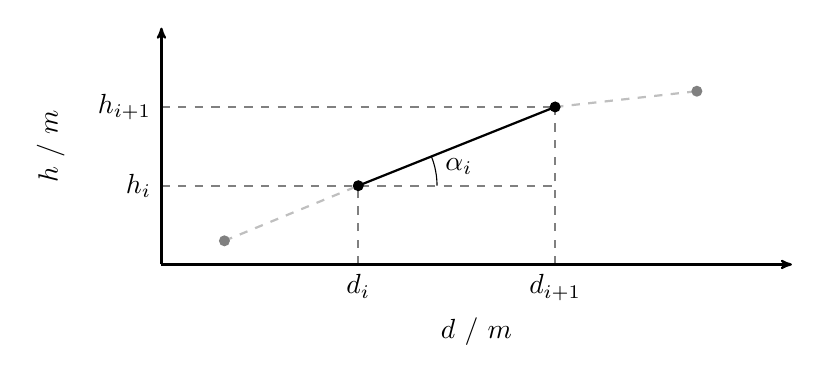
\begin{tikzpicture}[thick,>=stealth']
	% Origin
	\coordinate (Origin) at (0,0);
	% Data points
	\coordinate (i-1) at (0.8,0.3);
	\coordinate (i) at (2.5,1);
	\coordinate (i+1) at (5,2);
	\coordinate (i+2) at (6.8,2.2);
	\coordinate (baseLinePoint) at (5,1);
	
	% Helping vertical lines
	\draw[gray,dashed] let \p1=(i) in (\x1,0) node[below, black] {$d_i$} -- (i);
	\draw[gray,dashed] let \p1=(i+1) in (\x1,0) node[below, black] {$d_{i+1}$} -- (i+1);
	% Helping horizontal lines
	\draw[gray,dashed] let \p1=(i) in (0,\y1) node[left, black] {$h_i$} -- (baseLinePoint);
	\draw[gray,dashed] let \p1=(i+1) in (0,\y1) node[left, black] {$h_{i+1}$} -- (i+1);
%	\draw[gray] (i) -- (baseLinePoint);
%	\draw[gray,dashed, name intersections={rightHelpLine}] let \p1=(i+1) in (0,\y1) node[left, black] {$h_{i+1}$} -- (i+1);
%	\draw (i) -- (i+1 |- rightHelpLine);

	% Angle
	\tkzMarkAngle[thin](baseLinePoint,i,i+1)
	\tkzLabelAngle[pos=1.3](baseLinePoint,i,i+1){$\alpha_i$}
	
	% Axis
	\draw[->] (Origin) -- coordinate (x axis mid) (8,0);
	\draw[->] (Origin) -- coordinate (y axis mid) (0,3);
	% Axis labels
	\node[below=0.55] at (x axis mid) {$d$ / $\unit{m}$};
	\node[rotate=90,yshift=40pt] at (y axis mid) {$h$ / $\unit{m}$};
	
	% Data lines
	\draw [lightgray,dashed] (i-1) -- (i);
	\draw [black] (i) -- (i+1);
	\draw [lightgray,dashed] (i+1) -- (i+2);
	% Data dots
	\fill [gray] (i-1) circle (0.07cm);
	\fill [black] (i) circle (0.07cm);
	\fill [black] (i+1) circle (0.07cm);
	\fill [gray] (i+2) circle (0.07cm);
\end{tikzpicture}
	\caption{Graphical representation of the inclination estimation.}
	\label{fig:inclinationTriangle}
\end{figure}

The estimated inclination data is visualized in~\cref{fig:inclination}.
\begin{figure}[htbp]
	\centering
	% This file was created by matlab2tikz.
%
%The latest updates can be retrieved from
%  http://www.mathworks.com/matlabcentral/fileexchange/22022-matlab2tikz-matlab2tikz
%where you can also make suggestions and rate matlab2tikz.
%
%This file has been created via figure2tikz on 22-Dec-2022 21:10:56.
%
\begin{tikzpicture}

\begin{axis}[%
width=\textwidth,
height=0.3\textwidth,
xmin=0,
xmax=3000,
%xlabel style={font=\color{white!15!black}},
xtick={0,500,1000,1500,2000,2500,3000},
xticklabels={0,500,1000,1500,2000,2500,3000},
xlabel={Distance / km},
ymin=-3,
ymax=3,
%ylabel style={font=\color{white!15!black}},
ytick={-3,-2,-1,0,1,2,3},
yticklabels={-3,-2,-1,0,1,2,3},
ylabel={Inclination / °},
axis background/.style={fill=white},
grid=both,
]
\addplot [color=black, forget plot]
  table[]{img/inclination/inclination-1.tsv};
\end{axis}
\end{tikzpicture}%
	\caption{Estimated road inclination along the track.}
	\label{fig:inclination}
\end{figure}
%This last plot indicates that the track is never particularly steep. Hence,~\cref{eq:lvdFrollApprpx} and~\cref{eq:lvdFgravApprpx} could be used, resulting in a smaller simulation running time and improvement of the computational effort.


\subsection{Speed Limit}
To comply with traffic regulations, it is necessary to adhere to the maximum allowed speed at all times.~\Cref{fig:speedLimit} shows the speed limit as a function of distance.
\begin{figure}[htbp]
	\centering
	\begin{externalize}{speedLimit}
		% This file was created by matlab2tikz.
%
%The latest updates can be retrieved from
%  http://www.mathworks.com/matlabcentral/fileexchange/22022-matlab2tikz-matlab2tikz
%where you can also make suggestions and rate matlab2tikz.
%
%This file has been created via figure2tikz on 22-Dec-2022 21:36:06.
%
\begin{tikzpicture}

\begin{axis}[%
width=\textwidth,
height=0.3\textwidth,
xmin=0,
xmax=3000,
%xlabel style={font=\color{white!15!black}},
xtick={0,500,1000,1500,2000,2500,3000},
xticklabels={0,500,1000,1500,2000,2500,3000},
xlabel={Distance / km},
ymin=40,
ymax=140,
ylabel style={font=\color{white!15!black}},
ylabel={Speed limit / $\unitfrac{km}{h}$},
axis background/.style={fill=white},
grid=both,
]
\addplot [color=black, thick, forget plot]
  table[]{img/speedLimit/speedLimit-1.tsv};
\end{axis}
\end{tikzpicture}%
	\end{externalize}
	\caption{Maximal allowed driving speed along the track.}
	\label{fig:speedLimit}
\end{figure}
This visualization clearly shows that the majority of the track corresponds to a highway with relatively high speed limits. The downward spikes in the speed limit correspond to crossings of residential areas.


\newpage
\section{Meteorological Conditions}
\label{sec:modelingWeatherData}
In this section, the three weather variables influencing the models are presented: the global irradiance, ambient temperature, and wind speed characterized by intensity and direction.

Furthermore, since the route of the competition passes through three time zones in Australia, the time reference used in this report is based on the starting location in Darwin.


\subsection{Solar Global Irradiance}
To make the analysis of~\cref{chp:strategy} possible, the global irradiance data is taken from~\cite{irradianceData:2022webpage} as a function of time only. However, the usage of this high resolution data comes with the drawback that it is referred to a single specific year and not to more accurate mean values.

\Cref{fig:irradianceRace2020} shows the global irradiance as a function of time for the five October days of 2020, when the competition takes place.
\begin{figure}[htbp]
	\centering
	% This file was created by matlab2tikz.
%
%The latest updates can be retrieved from
%  http://www.mathworks.com/matlabcentral/fileexchange/22022-matlab2tikz-matlab2tikz
%where you can also make suggestions and rate matlab2tikz.
%
%This file has been created via figure2tikz on 20-Dec-2022 09:12:11.
%
\begin{tikzpicture}

\begin{axis}[%
width=\textwidth,
height=0.3\textwidth,
xmin=0,
xmax=7080,
%xlabel style={font=\color{white!15!black}},
xtick={0,1400,2850,4280,5720},
xticklabels={Oct 20,Oct 21,Oct 22,Oct 23,Oct 24},
xlabel={Time / days},
ymin=0,
ymax=1200,
%ylabel style={font=\color{white!15!black}},
ytick={0,300,600,900,1200},
yticklabels={0,300,600,900,1200},
ylabel={Global irradiance / $\unitfrac{W}{m^2}$},
axis background/.style={fill=white},
grid=both
]
\addplot [color=black, forget plot]
  table[]{img/irradianceRace2020/irradianceRace2020-1.tsv};
\end{axis}
\end{tikzpicture}%
	\caption{Data from the 20. October until 24. October 2020 of the global irradiance.}
	\label{fig:irradianceRace2020}
\end{figure}


\subsection{Ambient Temperature}
Ambient temperature data along the competition route is kindly provided by the \textit{Institute for Atmospheric and Climate Science} at ETH~\cite{weatherData:2022webpage}, and is given as mean values over the last fifty years, with hourly precision for time and distance every $\unit[5]{km}$. This data refers to temperatures measurement taken at $\unit[10]{m}$ above ground level.~\Cref{fig:ambientTemperature} shows the ambient temperature for three different time as a function of distance.
\begin{figure}[htbp]
	\centering
	\begin{externalize}{ambientTemperature}
		% This file was created by matlab2tikz.
%
%The latest updates can be retrieved from
%  http://www.mathworks.com/matlabcentral/fileexchange/22022-matlab2tikz-matlab2tikz
%where you can also make suggestions and rate matlab2tikz.
%
%This file has been created via figure2tikz on 10-Jan-2023 11:57:01.
%
\begin{tikzpicture}

\begin{axis}[%
width=\textwidth,
height=0.3\textwidth,
unbounded coords=jump,
xmin=0,
xmax=3000,
xlabel style={font=\color{white!15!black}},
xtick={0,500,1000,1500,2000,2500,3000},
xticklabels={0,500,1000,1500,2000,2500,3000},
xlabel={Distance / km},
ymin=0,
ymax=40,
ylabel style={font=\color{white!15!black}},
ylabel={Ambient Temperature / $\unit{\celsius}$},
axis background/.style={fill=white},
grid=both,
legend pos=south west,
legend cell align={left},
legend style={draw=none},
]
\addplot [cyan, thick]
  table[]{img/ambientTemperature/ambientTemperature-1-x04-30.tsv};
\addlegendentry{04:30}

\addplot [orange, thick]
  table[]{img/ambientTemperature/ambientTemperature-2-x13-30.tsv};
\addlegendentry{13:30}

\addplot [black, thick]
  table[]{img/ambientTemperature/ambientTemperature-3-x20-30.tsv};
\addlegendentry{20:30}

\end{axis}
\end{tikzpicture}%
	\end{externalize}
	\caption{Ambient temperature data for three different times of the day.}
	\label{fig:ambientTemperature}
\end{figure}
It is evident that the values tend to be similar at the beginning and at the end of the race. This is probably due to the fact that the proximity to the ocean mitigates the air temperature, whereas these differences are greater inland.


\subsection{Wind Speed}
\label{sec:windSpeed}
Both wind direction and intensity taken from~\cite{weatherData:2022webpage} influence the aerodynamic drag force as mentioned in~\cref{sec:modelLVD} and the generated power with the PV panels explained in~\cref{sec:modelPV}.

The vector decomposition needed to find the relevant values is shown in~\cref{fig:windSpeedVectors}~\cite{SolUTra:2006mt}.
\begin{figure}[htbp]
	\centering
		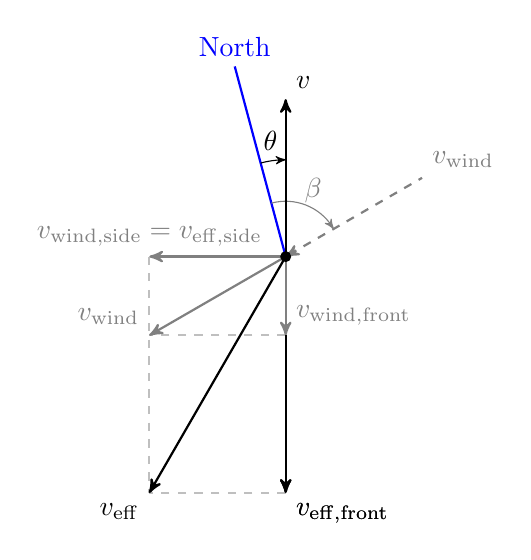
\begin{tikzpicture}[
	thick,
	>=stealth'
	]
	% Definition
	\def\angleWind{30}
	\def\angleNorth{105}
	
	\def\betragWind{2}
	\def\betragCar{2}
	\def\betragWindSide{\betragWind*cos(\angleWind)}
	\def\betragWindFront{\betragWind*sin(\angleWind)}
	\def\betragEffSide{\betragWindSide}
	\def\betragEffFront{\betragWindFront+\betragCar} %why not working?
	
	% Origin
	\coordinate (Origin) at (0,0);
	\coordinate (W) at (\angleWind:\betragWind); %for angle wind
	\coordinate (N) at (\angleNorth:\betragWind); %for angles
	\coordinate (V) at (0,\betragCar); %for angle car
	
	% North line
	\draw[blue] (Origin) -- (\angleNorth:2.5) node[above] {North};
	
	% Helping lines
	\draw[lightgray,dashed] (-{\betragEffSide},0) -- (-{\betragEffSide},-3);
	\draw[lightgray,dashed] (0,-{\betragWindFront}) -- (-{\betragWindSide},-{\betragWindFront});
	\draw[lightgray,dashed] (0,-3) -- (-{\betragEffSide},-3);
	
	% Angles
	\draw pic[<-,"$\beta$",draw=black,angle radius=20,angle eccentricity=1.3,thin,gray] {angle=W--Origin--N};
	\draw pic[<-,"$\theta$",draw=black,angle radius=35,angle eccentricity=1.2,thin,black] {angle=V--Origin--N};
	
	% Car vectors
	\draw[->,black] (Origin) -- (90:\betragCar) node[above right, black] {$v$};
	
	% Wind vectors
	\draw[<-,gray,dashed] (Origin) -- ({\angleWind}:{\betragWind}) node[above right] {$v_\mathrm{wind}$};
	\draw[->,gray] (Origin) -- ({180+\angleWind}:{\betragWind}) node[above left] {$v_\mathrm{wind}$};
	\draw[->,gray] (Origin) -- (180:{\betragWindSide}) node[above] {$v_\mathrm{wind,side} = v_\mathrm{eff,side}$};
	\draw[->,gray] (Origin) -- (270:{\betragWindFront}) node[above right] {$v_\mathrm{wind,front}$};
	
	% Effective wind vectors
	\draw[->,black,dashed] (0,{-\betragWindFront}) -- (270:{\betragEffFront})  node[below right] {$v_\mathrm{eff,front}$};
	\draw[->,black] (0,-{\betragWindFront}) -- (0,-3)  node[below right] {$v_\mathrm{eff,front}$};
	\draw[->,black] (Origin) -- ({-\betragWindSide},-3)  node[below left] {$v_\mathrm{eff}$};
	
%	\draw[->,black] (0,0) -- (3,0);
%	\draw[->,red,dashed] (0,0) -- ({\betragEffFront},0);
	
	% Origin dot
	\fill [black] (Origin) circle (0.07cm);
\end{tikzpicture}
	\caption{Vector representation of the relevant velocity components in coordinate system relative to the car driving direction pointing upwards. The angles are relative to the North Pole.}
	\label{fig:windSpeedVectors}
\end{figure}

First, the wind vector is decomposed into side wind and front wind relative to the car direction given by the velocity vector $\vec{v}$:
\begin{align}
	v_\mathrm{wind,side} &= \abs{\vec{v}_\mathrm{wind}} \cdot \sin\left(\beta - \theta \right) \\
	v_\mathrm{wind,front} &= \abs{\vec{v}_\mathrm{wind}} \cdot \cos\left(\beta - \theta \right)
\intertext{where $\vec{v}_\mathrm{wind}$ is the incident wind speed, $\beta$ is the angle of attack relative to the north, and $\theta$ is the angle of driving direction relative to the north. Second, the effective velocity is calculated considering its front and side contribution:}
	v_\mathrm{eff,side} &= v_\mathrm{wind,side} \\
	v_\mathrm{eff,front} &= v + v_\mathrm{wind,front} \\
	v_\mathrm{eff} &= \sqrt{v_\mathrm{eff,side}^2 + v_\mathrm{eff,front}^2}
\end{align}

As for the ambient temperature, also here the discrepancy of this data is improved with linear interpolation and the matching function.
%\begin{figure}[htbp]
%	\centering
%	\includegraphics[width=0.8\textwidth]{img/Windrose.pdf}
%	\caption{Wind data expressed in a windrose diagram.}
%	\label{fig:Windrose}
%\end{figure}
%\begin{figure}[htbp]
%	\centering
%	\pgfplotsset{
	polar bar/.style={
		scatter,
		draw=none,
		mark=none,
		visualization depends on=rawy\as\rawy,
		area legend,
		legend image code/.code={%
			\fill[##1] (0cm,-0.1cm) rectangle (0.6cm,0.1cm);
		},
		/pgfplots/scatter/@post marker code/.add code={}{
			\pgfmathveclen{\pgf@x}{\pgf@y}
			\edef\radius{\pgfmathresult}
			\fill[]
			(\pgfkeysvalueof{/data point/x},-\pgfkeysvalueof{/data point/y})
			++({\pgfkeysvalueof{/data point/x}-#1/2},\pgfkeysvalueof{/data point/y})
			arc [start angle=\pgfkeysvalueof{/data point/x}-#1/2,
			delta angle=#1,
			radius={\radius pt}
			]
			-- +({\pgfkeysvalueof{/data point/x}+#1/2},-\rawy)
			arc [start angle=\pgfkeysvalueof{/data point/x}+#1/2,
			delta angle=-#1,
			radius={
				(\pgfkeysvalueof{/data point/y} - \rawy) / \pgfkeysvalueof{/data point/y} * \radius pt
			}
			]
			--cycle;
		}
	},
	polar bar/.default=30
}

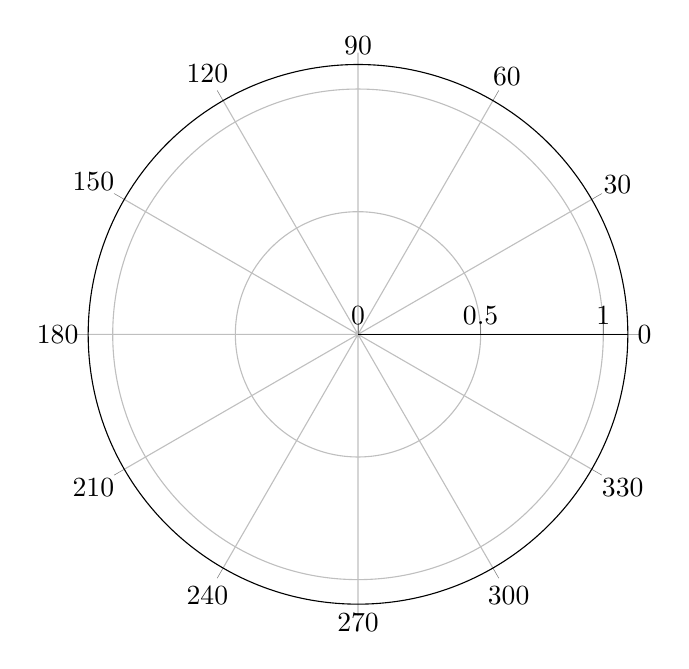
\begin{tikzpicture}
	\begin{polaraxis}[
		xtick={0,45,...,315},
%		xticklabels={E,NE,N,NW,W,SW,S,SE},
		ytick=\empty,
%		legend entries={0 to 0.5, 0.5 to 2, 2 to 4, 4 to 6},
%		cycle list={cyan!20, cyan!50, cyan, cyan!50!black, cyan!20!black},
%		legend pos=outer north east
		]
%		\pgfplotsinvokeforeach{1,...,6}{
%			\addplot +[polar bar=17, stack plots=y]
%			table [x expr=-\thisrowno{0}+90, y index=#1] {frequencies.csv};
%		}
	\end{polaraxis}
\end{tikzpicture}
%	\caption{TODO.}
%	\label{fig:windrose}
%\end{figure}

%\clearpage
\newpage
\section{Official Rules}
\label{sec:bwscRules}
The BWSC has its own specific rules that can be downloaded on this link~\cite{bwscRules:2022webpage}. Not only they shape the opportunities and challenges that arise in this competition, but also ignoring or violating them can result in penalties or disqualification. Thus, it is of high importance to take them into consideration when making decisions and developing a plan.

The list of relevant rules can be divided into three categories based on their domain of application: time, space, and general. In the following paragraphs, only the rules that are relevant to the objectives of this thesis are listed.

\paragraph{Time domain}
The rules in the time domain pertain to the timing of various actions and events, such as when it is allowed to drive or permitted to tilt the car deck towards the sun:
\begin{itemize}
	\item The driving time on Day 1 is allowed between 10:00 and 17:00 (Rule 3.20.1).
	\item The driving time after Day 1 is allowed between 08:00 and 17:00 (Rule 3.20.2).
	\item From 15 minutes before sunrise until 15 minutes after sunset, teams are allowed to tilt the deck of their car towards the sun to recharge the batteries (Rule 3.27.8).
\end{itemize}
\paragraph{Space domain}
The rules in the space domain relate to the physical location of the car and its actions, such as the maximum speed limit on different types of roads or the requirement to stop at certain locations:
\begin{itemize}
	\item There are nine control stops at fix locations, where every team must stop for 30 minutes. In the case that a control stop is reached after 16:30, the time difference has to be recovered the next day starting from 08:00. For instance, if a team stops at 16:50, the next day it can start driving at 08:20 (Rule 3.26.1).
	\item Teams must not drive faster than the maximal allowed speed (Rule 3.31.7).
\end{itemize}
\paragraph{General}
The general rules are not specific to either time or space, but rather apply to the competition as a whole:
\begin{itemize}
	\item Teams can start their race with fully charged batteries (Rule 1.5.2).
	\item Teams should be able to sustain a minimal driving speed for open road of at least $v_\mathrm{min} = \unitfrac[60]{km}{h}$ (Rule 3.29.1).
\end{itemize}


% !TeX spellcheck = en_US
% !TeX encoding = UTF-8
% !TeX root = ../report.tex

\chapter{Simulation of the Bridgestone World Solar Challenge}
\label{chp:simulation}
In this chapter, the BWSC simulation is presented exhaustively, from its general form to the description of individual blocks. The graphical block diagram representation clarify the Simulink interconnections and provides an understandable division between the components. The most general description is shown in~\cref{fig:simOverview}. The overall simulation is composed of three individual subsystems that explained in detail in~\cref{sec:simPlant,sec:simWeather,sec:simDriver}, following~\cref{sec:simPreparation} which provides information on Simulink and on the modification of the data presented in~\cref{sec:modelingWeatherData}.
\begin{figure}[htbp]
	\centering
	% Styles
\tikzstyle{block} = [rectangle, thick, minimum width=2.5cm, minimum height=1.5cm,text centered, text width=2cm, draw=black, fill=white]
\tikzstyle{arrow} = [thick, ->, >=stealth]

\begin{tikzpicture}
	
	% Blocks
	\matrix[column sep=1cm, row sep=1cm]{
	%first row
	&
	\coordinate (c12); &
	&
	\coordinate (c14); &
	&
	\\
	%second row
	\coordinate (c21); &
	\node[block] (driver) {Driver}; &
	&
	\node[block] (plant) {Plant}; &
	\coordinate (c25); &
	\\
	%third row
	&
	&
	\coordinate (c33); &
	\node[block] (weather) {Weather}; &
	\coordinate (c35); &
	\\
	};

	% Arrows
	\draw[arrow] (c21) -- (driver);
	\draw[arrow] (c33) -- (weather);
	\draw[arrow] (driver) -- (plant);
	\draw[arrow] (weather) -- (plant);
	\draw[arrow] (plant) -- (c25) -- (c35) -- (weather);
	\draw[arrow] (plant) -- (c14) -- (c12) -- (driver);
	

\end{tikzpicture}
	\caption{Block diagram of the main components of the Simulink simulation. The arrows exclusively show the relations between blocks and not the signals they exchange.}
	\label{fig:simOverview}
\end{figure}

Additional blocks are used to store data and stop the simulation once the finish line in Adelaide is passed.

\newpage
\section{Preparation}
\label{sec:simPreparation}
A dynamic approach is preferred for the simulation because the objective of the simulation is to provide information about the resulting total racing time for a given set of inputs. In fact, a quasi-static approach is not suitable because it needs a real velocity profile as an input instead of as an output, which would require the total racing time to be predetermined.

One important aspect of the simulation implementation is that Simulink is based on an absolute time in seconds $t_\mathrm{sim}$. As a result, the data for time must be preprocessed accordingly in Matlab. Specifically, data for times when the car is stopped and there is no sunlight (i.e. nights) is removed. The remaining vector is converted to a monotonically increasing time scale in seconds. Additionally, as discussed in~\cref{sec:bwscRules}, it is possible to tilt the car deck towards the sun from 17:00 to 08:00, which increases the amount of solar radiation that hits the PV panels. This effect is taken into account by multiplying the global irradiance with a correction factor that is estimated using the plots in~\cite{BuckBoost:2021article}. Its value is 1.8, meaning that the irradiance of~\cref{fig:irradianceRace2020} is increased by 1.8 times from 17:00 to 08:00. These modifications are shown in~\cref{fig:irradianceSimulation2020}, where the global irradiance data is now suitable for the simulation $G_\mathrm{sim}$.
\begin{figure}[htbp]
	\centering
	\begin{externalize}{irradianceSimulation2020}
		% This file was created by matlab2tikz.
%
%The latest updates can be retrieved from
%  http://www.mathworks.com/matlabcentral/fileexchange/22022-matlab2tikz-matlab2tikz
%where you can also make suggestions and rate matlab2tikz.
%
%This file has been created via figure2tikz on 28-Dec-2022 21:48:38.
%
\begin{tikzpicture}

\begin{axis}[%
width=\textwidth,
height=0.3\textwidth,
xmin=0,
xmax=131340,
%xlabel style={font=\color{white!15!black}},
xtick={0,32500,82000,131340},
xticklabels={0,32500,82000,131340},
xlabel={Simulation time / s},
ymin=0,
ymax=1200,
%ylabel style={font=\color{white!15!black}},
ytick={0,300,600,900,1200},
yticklabels={0,300,600,900,1200},
ylabel={Global irradiance / $\unitfrac{W}{m^2}$},
axis background/.style={fill=white},
grid=both,
scaled x ticks = false,
x tick label style={/pgf/number format/fixed},
]
\addplot [color=black, forget plot]
  table[]{img/irradianceSimulation2020/irradianceSimulation2020-1.tsv};
\end{axis}
\end{tikzpicture}%
	\end{externalize}
	\caption{Global irradiance plot from the 22. October until 24. October 2020 obtained with correcting factor when standing and cut during the nights. The vertical grid lines represent the day change.}
	\label{fig:irradianceSimulation2020}
\end{figure}

Similar conversion to absolute time are performed for both ambient temperature and wind data.

\newpage
\section{Plant}
\label{sec:simPlant}
The mathematical models derived in the previous chapter represent the foundation for the implementation of the Plant components. A subdivision into the four subsystems - LVD, Motor, PV, and Battery - is natural and will help reducing the complexity. From~\cref{sec:simLVD} to~\cref{sec:simBattery} each of the blocks are explained in more detail. A schematic illustration of the relation between them in the Plant subsystem is shown in~\cref{fig:simPlant}. 
\begin{sidewaysfigure}[htbp]
	\centering
	% Styles
\tikzset{
	smallBlock/.style = {rectangle, thick, minimum width=0.8cm, minimum height=0.8cm,text centered, draw=black, fill=white},
	midBlock/.style = {rectangle, thick, minimum width=2cm, minimum height=1.5cm,text centered, text width=3cm, draw=black, fill=white},
	bigBlock/.style = {rectangle, thick, minimum width=2cm, minimum height=2.5cm,text centered, text width=2cm, draw=black, fill=white},
	arrow/.style= {thick, black, ->, >=stealth},
	line/.style= {thick, black},
	textOutput/.style = {black,right},
	textInput/.style = {black,left},
	container/.style = {gray,dashed},
	sum/.style = {circle, minimum size=0.7cm, thick, draw=black, fill=white},
	%sum
	charge node/.style={inner sep=0pt},
	pics/sum block/.style n args={4}{
		code={
			\path node (n) [draw, circle, inner sep=0pt, minimum size=0.7cm] {}
			(n.north) +(0,-1.5mm) node [charge node] {$#1$}
			(n.south) +(0,1.5mm) node [charge node] {$#2$}
			(n.west) +(1.5mm,0) node [charge node] {$#3$}
			(n.east) +(-1.5mm,0) node [charge node] {$#4$}
			;
		}
	}
}
\begin{tikzpicture}
	% Definition
	%for three arrows
	\def\up{0.7}
	\def\down{-\up}
	\def\right{0.7}
	\def\left{-\right}
	%for two arrows
	\def\UP{0.5}
	\def\DOWN{-\UP}
	\def\RIGHT{0.5}
	\def\LEFT{-\RIGHT}
	%radius
	\def\radius{0.07}
	
	% Blocks
	\matrix[column sep=0.65cm, row sep=0.8cm]{
		%first row
		& \coordinate (c12); & & & &  & & & & &  & & & &
		\\
		%second row
		& & & & &  & \coordinate (c27); & & & &  \node[midBlock] (inclination) {$\alpha(d)$ \\ 1D Look-up Table}; & \coordinate (c212); & & &
		\\
		%third row
		& & \coordinate (c33); & & \coordinate (c35); &  & \coordinate (c37); & & & \coordinate (c310); &  & & & \coordinate (c314); &
		\\
		%fourth row
		\coordinate (c41); & & \coordinate (c43); & & \coordinate (c45); &  & \node[bigBlock] (lvd) {LVD}; & \node[smallBlock] (mass) {$\frac{1}{m_\mathrm{tot}}$}; & \node[smallBlock] (intAcc) {$\int$}; & \coordinate (c410); &  \node[smallBlock] (intVel) {$\int$}; & \coordinate (c412); & & \coordinate (c414); &
		\\
		%fifth row
		\coordinate (c51); & & & & \node[bigBlock] (motor) {Motor}; &  & \coordinate (c57); & \node[sum] (sum) {}; & & &  \node[midBlock, minimum height=1cm] (battery) {Battery}; & & & \coordinate (c514); &
		\\
		%sixth row
		\coordinate (c61); & & \node[bigBlock] (PV) {PV}; & & \coordinate (c65); &  & & \coordinate (c68); & & &  & & & &
		\\
		%seventh row
		& & & & &  & & & & &  & & \coordinate (c713); & &
		\\
	};
	
	% Container
	\draw[container] (c12) rectangle (c713);
	\node[gray, anchor=north west] at (c12.north west) {Plant};
	
	% Arrows;
	%to second row
	\draw[arrow] (c212) -- (inclination);
	\draw[line] (c412) -- (c212);
	\draw[line] (inclination) -- ([xshift=\RIGHT cm]c27) node[midway, above] {$\alpha$};
	%to third row
	\draw[arrow] ([xshift=\RIGHT cm]c33) -- (c314) node[textOutput] {$v$};
	\draw[line] (c410) -- (c310);
	\draw[arrow] ([xshift=\RIGHT cm]c27) -- ([xshift=\RIGHT cm]lvd.north);
	%to fourth row
	\draw[arrow] (c412) -- (c414) node[textOutput] {$d$};
	\draw[line] (intVel) -- (c412) node[midway, above] {$d$};
	\draw[arrow] ([yshift=\DOWN cm]c41) node[textInput, text width=1.8cm, text centered] {Stop force is decided} -- ([yshift=\DOWN cm]lvd.west);
	\draw[arrow] ([yshift=\UP cm]c41) node[textInput] {$v_\mathrm{wind,front}$} -- ([yshift=\UP cm]lvd.west);
	\draw[arrow] ([xshift=\LEFT cm]c37) -- ([xshift=\LEFT cm]lvd.north);
	\draw[arrow] (lvd) -- (mass);
	\draw[arrow] (mass) -- (intAcc) node[midway, above] {$a$};
	\draw[line] (intAcc) -- (c410) node[midway, above] {$v$};
	\draw[arrow] (c410) -- (intVel);
	\draw[arrow] ([yshift=\up cm]c57) -- (lvd);
	%to fifth row
	\draw[arrow] (battery) -- (c514) node[textOutput] {$x_\mathrm{SoC}$};
	\draw[arrow] (motor) -- (sum) node[midway, above] {$P_\mathrm{mot,el}$};
	\draw[arrow] (sum) -- (battery) node[midway, above] {$P_\mathrm{bat}$};
	\draw[arrow] ([xshift=\RIGHT cm]c35) -- ([xshift=\RIGHT cm]motor.north);
	\draw[arrow] (c68) -- (sum);
	\draw[line] (PV) -- (c65) node[midway, above] {$P_\mathrm{PV}$};
	\draw[arrow] (c65) -- (motor);
	\draw[arrow] (c51) node[textInput] {$F_\mathrm{trac,req}$} -- (motor.west);
	\draw[arrow] ([xshift=\LEFT cm, yshift=\DOWN cm]c45) -- ([xshift=\LEFT cm]motor.north);
	\draw[arrow] ([yshift=\down cm]motor.east) -- ([yshift=\down cm]c514) node[textOutput] {$F_\mathrm{trac,lim}$};
	\draw[line] ([yshift=\up cm]motor.east) -- ([yshift=\up cm]c57) node[midway, above] {$F_\mathrm{trac}$};
	%to sixth row
	\draw[arrow] (c61) node[textInput] {$T_\mathrm{amb}$} -- (PV);
	\draw[arrow] ([xshift=\RIGHT cm]c33) -- ([xshift=\RIGHT cm]PV.north);
	\draw[line] (PV) -- (c68);
	\draw[arrow] ([yshift=\up cm]c61) node[textInput] {$G_\mathrm{sim}$} -- ([yshift=\up cm]PV.west);
	\draw[arrow] ([yshift=\down cm]c61) node[textInput] {$v_\mathrm{wind,side}$} -- ([yshift=\down cm]PV.west);
	\draw[arrow] ([yshift=\UP cm, xshift=\LEFT cm]c43) -- ([xshift=\LEFT cm]PV.north);
	
	% Dots
	\fill [black] (c310) circle (\radius cm);
	\fill [black] ([xshift=\RIGHT cm]c35) circle (\radius cm);
	\fill [black] ([xshift=\LEFT cm]c37) circle (\radius cm);
	
	\fill [black] (c410) circle (\radius cm);
	\fill [black] (c412) circle (\radius cm);
	\fill [black] ([xshift=\LEFT cm, yshift=\DOWN cm]c45) circle (\radius cm);
	\fill [black] ([xshift=\LEFT cm, yshift=\UP cm]c43) circle (\radius cm);
	
	\fill [black] (c65) circle (\radius cm);
	
	%sum
	\path pic at (sum) {sum block={}{-}{+}{}};
	
\end{tikzpicture}
	\caption{Block diagram representation for the Plant.}
	\label{fig:simPlant}
\end{sidewaysfigure}
Here, six inputs are received, whereas four outputs are generated, as listed in~\cref{tab:simInOutPlant}.
\begin{table}[htbp]
	\centering
	\caption{Input/Output signals for the Plant.}
	\label{tab:simInOutPlant}
	
	\begin{tabular}{c l l l l}
		\toprule
		& Block & Signal & Symbol & Type \\ 
		\midrule
		\multirow{6}{*}{Input from}
		& Driver & Requested traction force & $F_\mathrm{trac,req}$ & Float \\
		& Driver & Stop force is decided & -- & Binary \\
		& Weather & Global irradiance & $G_\mathrm{sim}$ & Float \\
		& Weather & Ambient temperature & $T_\mathrm{amb}$ & Float \\
		& Weather & Side wind speed & $v_\mathrm{wind,side}$ & Float \\
		& Weather & Frontal wind speed & $v_\mathrm{wind,front}$ & Float \\

		\midrule
		\multirow{4}{*}{Output to}
		& Weather and Driver & Car velocity & $v$ & Float \\
		& Weather and Driver & Driven distance & $d$ & Float \\
		& Driver & SoC & $x_\mathrm{SoC}$ & Float \\
		& Driver & Traction force bounds & $F_\mathrm{trac,lim}$ & Float \\
		\bottomrule
	\end{tabular}
\end{table}

The other important building blocks of the Plant shown in the figure are the following:
\begin{itemize}
	\item A one dimensional \texttt{Look-up Table} that interpolates the distance traveled from the starting line to obtain the route inclination;
	\item A \texttt{Gain} block that receives the inertial force $m_\mathrm{tot} \frac{d}{dt} v(t)$ from LVD and outputs the car acceleration;
	\item Two \texttt{Integrators} in series to generate the actual car velocity and position. Both initial conditions are set to zero, representing a standing start of the race; and
	\item A \texttt{Sum} block that guarantees that the power balance equation of~\cref{sec:modelPowerBalance} is fulfilled.
\end{itemize}


\subsection{Longitudinal Vehicle Dynamics}
\label{sec:simLVD}
The \texttt{Subsystem} for the LVD includes the implementation of the equations described in~\cref{sec:modelLVD}. The road inclination is taken into account, and the forces of rolling resistance $F_\mathrm{roll}$ and gravity $F_\mathrm{grav}$ are not approximated. For this reason, five inputs are necessary, while there is only one output, as listed in~\cref{tab:simInOutLVD}.
\begin{table}[htbp]
	\centering
	\caption{Input/Output signals for the LVD.}
	\label{tab:simInOutLVD}
	
	\begin{tabular}{c l l l l}
		\toprule
		& Block & Signal & Symbol & Type \\ 
		\midrule
		\multirow{5}{*}{Input from}
		& -- & Road inclination & $\alpha$ & Float \\
		& Weather & Car velocity & $v$ & Float \\
		& Weather & Frontal wind speed & $v_\mathrm{wind,front}$ & Float \\
		& Driver & Stop force is decided & -- & Binary \\
		& Motor & Traction force & $F_\mathrm{trac}$ & Float \\
		\midrule
		\multirow{1}{*}{Output to}
		& Internal & Inertial force & $m_\mathrm{tot} \frac{d}{dt} v(t)$ & Float \\
		\bottomrule
	\end{tabular}
\end{table}

The LVD implementation differs from the modeling equations by an additional friction force created with a \texttt{Coulomb \& Viscous Friction} block. It is turned on with the boolean signal \enquote{Stop force is decided} from the Driver, which at the same time deactivates the other friction forces. This corresponds to the effect of activating a hand brake system, necessary to keep the velocity at a constant zero during the control and overnight stops without consuming electrical power.


\subsection{Electric Motor}
\label{sec:simMotor}
This \texttt{Subsystem} is divided into two parts: the first one calculates the bounds used in the Controllers \texttt{Subsystem} of~\cref{sec:simDriver}, while the second one contains the model equations.

Four inputs are received and three outputs generated, as listed in~\cref{tab:simInOutMotor}.
\begin{table}[htbp]
	\centering
	\caption{Input/Output signals for the Motor.}
	\label{tab:simInOutMotor}
	
	\begin{tabular}{c l l l l}
		\toprule
		& Block & Signal & Symbol & Type \\ 
		\midrule
		\multirow{4}{*}{Input from}
		& -- & Car velocity & $v$ & Float \\
		& Driver & Stop force is decided & -- & Binary \\
		& Driver & Requested traction force & $F_\mathrm{trac,req}$ & Float \\
		& PV & PV power & $P_\mathrm{PV}$ & Float \\
		\midrule
		\multirow{3}{*}{Output to}
		& LVD & Traction force & $F_\mathrm{trac}$ & Float \\
		& Sum & Electric motor power & $P_\mathrm{mot,el}$ & Float \\
		& Driver & Traction force bounds & $F_\mathrm{trac,lim}$ & Float \\
		\bottomrule
	\end{tabular}
\end{table}


\paragraph{Bounds Calculator}
This \texttt{MATLAB Function} contains the codes that generates the maximal and minimal mechanical torque that can be provided by the electric motor. These values are determined by considering all the limits of the motor described in~\cref{sec:modelMotor} and the battery limits from~\cref{sec:modelBattery}. The integration of these limits requires rewriting~\cref{eq:powerBalance} for the electric motor power, which leads to the following upper bounds:
\begin{align}
	P_\mathrm{mot,el} &\leq P_\mathrm{bat,max} + P_\mathrm{PV}, \\
	P_\mathrm{mot,el} &\leq I_\mathrm{bat,max} \cdot \left( U_\mathrm{bat,oc} - R_\mathrm{bat} \cdot I_\mathrm{bat,max} \right) + P_\mathrm{PV}, \\
	P_\mathrm{mot,el} &\leq \frac{U_\mathrm{bat,oc}^2}{4 \cdot R_\mathrm{bat}} + P_\mathrm{PV}.
\end{align}
While for the lower limits holds:
\begin{align}
	P_\mathrm{mot,el} &\geq P_\mathrm{bat,min} + P_\mathrm{PV}, \\
	P_\mathrm{mot,el} &\geq I_\mathrm{bat,min} \cdot \left( U_\mathrm{bat,oc} - R_\mathrm{bat} \cdot I_\mathrm{bat,min} \right) + P_\mathrm{PV}.
\end{align}
Furthermore, numerical problems arise when dividing with a velocity approaching zero to convert power to forces or torques. For this reason, \texttt{Saturation} blocks and explicit division with a small number is implemented. The torque signals are converted to forces and sent to the Driver block as $F_\mathrm{trac,lim}$.

\paragraph{Motor}
The modeling equations derived in~\cref{sec:modelMotor} are written in this \texttt{MATLAB Function}, including the limits and the torque bounds calculated in the Bounds Calculator.

In case of strong braking, not all the power can be recuperated in the battery. Therefore, a dissipative braking force is also calculated here.


\subsection{PV Module}
\label{sec:simPV}
In this subsystem, the model derived in~\cref{sec:modelPV} is included in a \texttt{MATLAB Function}. Five inputs are received, while only one output is generated, as listed in~\cref{tab:simInOutPV}.
\begin{table}[htbp]
	\centering
	\caption{Input/Output signals for the PV.}
	\label{tab:simInOutPV}
	
	\begin{tabular}{c l l l l}
		\toprule
		& Block & Signal & Symbol & Type \\ 
		\midrule
		\multirow{5}{*}{Input from}
		& -- & Car velocity & $v$ & Float \\
		& Weather & Frontal wind speed & $v_\mathrm{wind,front}$ & Float \\
		& Weather & Global irradiance & $G_\mathrm{sim}$ & Float \\
		& Weather & Ambient temperature & $T_\mathrm{amb}$ & Float \\
		& Weather & Side wind speed & $v_\mathrm{wind,side}$ & Float \\
		\midrule
		\multirow{1}{*}{Output to}
		& Motor and sum & PV power & $P_\mathrm{PV}$ & Float \\
		\bottomrule
	\end{tabular}
\end{table}

\subsection{Battery Pack}
\label{sec:simBattery}
The model of the battery pack described in~\cref{sec:modelBattery} is implemented in Simulink using a series of basic blocks. The model begins with a \texttt{MATLAB function} block, followed by an \texttt{Integrator} block to calculate the actual charge, a \texttt{Gain} block to determine the SoC, and a \texttt{Saturation} block to prevent the SoC from exceeding the limit of $\unit[100]{\%}$. Any additional power supplied to the battery after this limit is reached, is assumed to be converted into heat.

As previously mentioned, the battery limits are not included in this subsystem, but rather in the electric motor block of~\cref{sec:simMotor}. This is necessary to ensure that the causality of the Simulink simulation is preserved.

Only one input is received, and one output is generated as listed in~\cref{tab:simInOutBattery}.
\begin{table}[htbp]
	\centering
	\caption{Input/Output signals for the Battery.}
	\label{tab:simInOutBattery}
	
	\begin{tabular}{c l l l l}
		\toprule
		& Block & Signal & Symbol & Type \\ 
		\midrule
		\multirow{1}{*}{Input from}
		& Sum & Battery power & $P_\mathrm{bat}$ & Float \\
		\midrule
		\multirow{1}{*}{Output to}
		& Controllers & SoC & $x_\mathrm{SoC}$ & Float \\
		\bottomrule
	\end{tabular}
\end{table}

\newpage
\section{Weather}
\label{sec:simWeather}
The analysis of the weather data of~\cref{sec:modelingWeatherData} and their conversion in seconds allow the implementation of this component with the mere usage of \texttt{Look-up Tables}: two dimensional tables are needed for the ambient temperature and wind speeds, while a one dimensional one is used for the global irradiance.~\Cref{fig:simWeather} shows the block diagram representation of this \texttt{Subsystem}, where the interpolations take place.

Two inputs are received, whereas four outputs are generated as listed in~\cref{tab:simInOutWeather}.
\begin{table}[htbp]
	\centering
	\caption{Input/Output signals for the Weather.}
	\label{tab:simInOutWeather}
	
	\begin{tabular}{c l l l l}
		\toprule
		& Block & Signal & Symbol & Type \\ 
		\midrule
		\multirow{2}{*}{Input from}
		& Simulink & Absolute time & $t_\mathrm{sim}$ & Float \\
		& Plant & Driven distance & $d$ & Float \\
		\midrule
		\multirow{4}{*}{Output to}
		& Plant & Global irradiance & $G_\mathrm{sim}$ & Float \\
		& Plant & Ambient temperature & $T_\mathrm{amb}$ & Float \\
		& Plant & Side wind speed & $v_\mathrm{wind,side}$ & Float \\
		& Plant & Frontal wind speed & $v_\mathrm{wind,front}$ & Float \\
		\bottomrule
	\end{tabular}
\end{table}

\begin{figure}[htbp]
	\centering
	% Styles
\tikzstyle{block} = [rectangle, thick, minimum width=2.5cm, minimum height=1.5cm,text centered, text width=3cm, draw=black, fill=white]
\tikzstyle{arrow} = [thick, ->, >=stealth]
\tikzstyle{textOutput} = [black,right]
\tikzstyle{textInput} = [black,left]
\tikzstyle{container} = [gray,dashed]

\begin{tikzpicture}
	% Definition
	\def\up{0.3}
	\def\down{-\up}
	\def\radius{0.07}
	
	% Blocks
	\matrix[column sep=1cm, row sep=0.5cm]{
		%first row
		& \coordinate (c12); & & & & & &
		\\
		%second row
		\coordinate (c21); & & & \coordinate (c24); & \node[block] (G) {$G_\mathrm{sim}(t_\mathrm{sim})$ \\ 1D Look-up Table}; & & \coordinate (c27); &
		\\
		%third row
		\coordinate (c31); & & \coordinate (c33); & \coordinate (c34); & \node[block] (T) {$T_\mathrm{amb}(d,t_\mathrm{sim})$ \\ 2D Look-up Table}; & & \coordinate (c37); &
		\\
		%fourth row
		& & \coordinate (c43); & \coordinate (c44); & \node[block] (vs) {$v_\mathrm{wind,side}(d,t_\mathrm{sim})$ \\ 2D Look-up Table}; & & \coordinate (c47); &
		\\
		%fifth row
		& & \coordinate (c53); & \coordinate (c54); & \node[block] (vf) {$v_\mathrm{wind,front}(d,t_\mathrm{sim})$ \\ 2D Look-up Table}; & & \coordinate (c57); &
		\\
		%sixth row
		& & & & & \coordinate (c66); & &
		\\
	};
	
	% Container
	\draw[container] (c12) rectangle (c66);
	\node[gray, anchor=north west] at (c12.north west) {Weather};
	
	% Arrows
	\draw[arrow] (c21) node[textInput] {$t_\mathrm{sim}$} -- (G);
	\draw[arrow] (G) -- (c27) node[textOutput] {$G_\mathrm{sim}$};
	
	\draw[arrow] ([yshift=\down cm]c31) node[textInput] {$d$} -- ([yshift=\down cm]T.west);
	\draw[arrow] (T) -- (c37) node[textOutput] {$T_\mathrm{amb}$};
	\draw[arrow] ([yshift=\up cm]c34) -- ([yshift=\up cm]T.west);
	
	\draw[arrow] (vs) -- (c47) node[textOutput] {$v_\mathrm{wind,side}$};
	\draw[arrow] ([yshift=\up cm]c44) -- ([yshift=\up cm]vs.west);
	\draw[arrow] ([yshift=\down cm]c43) -- ([yshift=\down cm]vs.west);
	
	\draw[arrow] (vf) -- (c57) node[textOutput] {$v_\mathrm{wind,front}$};
	\draw[arrow] ([yshift=\down cm]c33) -- ([yshift=\down cm]c53) -- ([yshift=\down cm]vf.west);
	\draw[arrow] (c24) -- ([yshift=\up cm]c54) -- ([yshift=\up cm]vf.west);
	
	% Dots
	\fill [black] (c24) circle (\radius cm);
	
	\fill [black] ([yshift=\up cm]c34) circle (\radius cm);
	\fill [black] ([yshift=\down cm]c33) circle (\radius cm);
	
	\fill [black] ([yshift=\up cm]c44) circle (\radius cm);
	\fill [black] ([yshift=\down cm]c43) circle (\radius cm);

	
\end{tikzpicture}
	\caption{Block diagram representation for the Weather.}
	\label{fig:simWeather}
\end{figure}

Alternatives to \texttt{Look-up Tables} are discarded because of the their slower computational performance with respect to these Simulink built-in blocks. Direct interpolation in Matlab and the usage of \texttt{Gridded Interpolant} were tested.

\newpage
\section{Driver}
\label{sec:simDriver}
The last of the three main components is the Driver, which is composed of a Decision Maker, a Controllers \texttt{Subsystem}, and three one dimensional \texttt{Look-up Tables}, as illustrated in~\cref{fig:simDriver}. The first table outputs the speed limit $v_\mathrm{max}$ at the current car position on the route, the second one provides the number of the current race day (day one is the 20. October), and the third outputs \enquote{true} when driving during the day is possible, namely from 10:00 to 17:00 on day one and from 08:00 to 17:00 for the rest of the race.
\begin{sidewaysfigure}[htbp]
	\centering
	% Styles
\tikzset{
	lookBlock/.style = {rectangle, thick, minimum width=2.5cm, minimum height=1.5cm,text centered, text width=3cm, draw=black, fill=white},
	block/.style = {rectangle, thick, minimum width=2.5cm, minimum height=1.5cm,text centered, text width=2.5cm, draw=none, fill=white},
	arrow/.style= {thick, black, ->, >=stealth},
	line/.style= {thick, black},
	textOutput/.style = {black,right},
	textInput/.style = {black,left},
	container/.style = {gray,dashed}
}

\begin{tikzpicture}
	% Definition
	%for three arrows
	\def\right{0.8}
	\def\left{-\right}
	%for two arrows
	\def\UP{0.55}
	\def\DOWN{-\UP}
	%radius
	\def\radius{0.07}
	
	% Blocks
	\matrix[column sep=1.3cm, row sep=0.7cm]{
		%first row
		& \coordinate (c12); & & & &  & & & & &
		\\
		%second row
		\coordinate (c21); & & & & &  & & \node[block] (C1) {}; & & &
		\\
		%third row
		\coordinate (c31); & & \coordinate (c33); & & &  & \coordinate (c37); & \node[block] (C2) {}; & & &
		\\
		%fourth row
		\coordinate (c41); & & & \coordinate (c44); & &  \coordinate (c46); & \coordinate (c47); & \node[block] (C3) {}; & & \coordinate (c410); &
		\\
		%fifth row
		& & & \coordinate (c54); & \node[lookBlock] (MS) {$v_\mathrm{max}(d)$ \\ 1D Look-up Table}; &  \coordinate (c56); & \node[block] (D1) {}; & \node[block] (C4) {}; & & &
		\\
		%sixth row
		& & \coordinate (c63); & & \node[lookBlock] (DN) {Day number$(t_\mathrm{sim})$ \\ 1D Look-up Table}; &  & \node[block] (D2) {}; & \node[block] (C5) {}; & & &
		\\
		%seventh row
		& & \coordinate (c73); & & \node[lookBlock] (Driving) {Driving is needed$(t_\mathrm{sim})$ \\ 1D Look-up Table}; &  & \node[block] (D3) {}; & \node[block] (C6) {}; & & &
		\\
		%eigth row
		& & & & &  & \coordinate (c87); & & & \coordinate (c810); &
		\\
		%ninth row
		& & & & &  & & & \coordinate (c99); & &
		\\
	};
	
	% Container
	\draw[container] (c12) rectangle (c99);
	\node[gray, anchor=north west] at (c12.north west) {Driver};
	
	% Arrows
	%to second
	\draw[arrow] ([yshift=\UP cm]c21) node[textInput] {$x_\mathrm{SoC}$} -- ([yshift=\UP cm]C1.west);
	\draw[arrow] ([yshift=\DOWN cm]c21) node[textInput] {$F_\mathrm{trac,lim}$} -- ([yshift=\DOWN cm]C1.west);
	%to third
	\draw[arrow] ([yshift=\UP cm]c31) node[textInput] {$v$} -- ([yshift=\UP cm]C2.west);
	\draw[arrow] ([yshift=\DOWN cm]c31) node[textInput] {$t_\mathrm{sim}$} -- ([yshift=\DOWN cm]C2.west);
	%to fourth
	\draw[arrow] ([yshift=\DOWN cm]C3.east) -- ([yshift=\DOWN cm]c410) node[textOutput] {$F_\mathrm{trac,req}$};
	\draw[arrow] ([yshift=\UP cm]c41) node[textInput] {$d$} -- ([yshift=\UP cm]C3.west);
	\draw[arrow] ([yshift=\DOWN cm]c46) -- ([yshift=\DOWN cm]C3.west);
	%to fifth
	\draw[line] ([yshift=\UP cm]c44) -- (c54);
	\draw[arrow] (c54) -- (MS);
	\draw[line] (MS) -- (c56) node[midway, above] {$v_\mathrm{max}$};
	\draw[arrow] (c56) -- (D1);
	\draw[line] ([yshift=\DOWN cm]c46) -- (c56);
	\draw[arrow] (D1) -- (C4) node[midway, above, text width=1.2cm, text centered] {Acc is dec};
	\draw[arrow] ([yshift=\UP cm, xshift=\left cm]c47) -- ([xshift=\left cm]D1.north);
	\draw[arrow] ([yshift=\DOWN cm]c37) -- (D1);
	\draw[arrow] ([yshift=\UP cm, xshift=\right cm]c37) -- ([xshift=\right cm]D1.north);
	%to sixth
	\draw[arrow] (c63) -- (DN);
	\draw[arrow] (DN) -- (D2);
	\draw[arrow] (D2) -- (C5) node[midway, above, text width=1.2cm, text centered] {Dec is dec};
	%to seventh
	\draw[line] ([yshift=\DOWN cm]c33) -- (c73);
	\draw[arrow] (c73) -- (Driving);
	\draw[arrow] (Driving) -- (D3);
	\draw[arrow] (D3) -- (C6) node[midway, above, text width=1.2cm, text centered] {Cruise is dec};
	%to eigth
	\draw[line] (D3) -- (c87);
	\draw[arrow] (c87) -- (c810) node[textOutput, text width=1.8cm, text centered] {Stop force is decided};
	
	% Dots
	\fill [black] ([yshift=\DOWN cm]c33) circle (\radius cm);
	\fill [black] ([yshift=\DOWN cm]c37) circle (\radius cm);
	\fill [black] ([yshift=\UP cm, xshift=\right cm]c37) circle (\radius cm);
	
	\fill [black] ([yshift=\UP cm]c44) circle (\radius cm);
	\fill [black] ([yshift=\UP cm, xshift=\left cm]c47) circle (\radius cm);
	
	\fill [black] (c56) circle (\radius cm);
	
	\fill [black] (c63) circle (\radius cm);
	
	%Fit
	\node [inner sep=-0.5\pgflinewidth,fit=(D1)(D2)(D3), draw] {Decision \\ Maker};
	\node [inner sep=-0.5\pgflinewidth,fit=(C1)(C2)(C3)(C4)(C5)(C6), draw] {Controllers};
	
	
\end{tikzpicture}
	\caption{Block diagram representation of the Driver.}
	\label{fig:simDriver}
\end{sidewaysfigure}

Five inputs are received, whereas two outputs are generated, as listed in~\cref{tab:simInOutDriver}.
\begin{table}[htbp]
	\centering
	\caption{Input/Output signals for the Driver.}
	\label{tab:simInOutDriver}
	
	\begin{tabular}{c l l l l}
		\toprule
		& Block & Signal & Symbol & Type \\ 
		\midrule
		\multirow{5}{*}{Input from}
		& Plant & SoC & $x_\mathrm{SoC}$ & Float \\
		& Plant & Traction force bounds & $F_\mathrm{trac,lim}$ & Float \\
		& Plant & Car velocity & $v$ & Float \\
		& Simulink & Absolute time & $t_\mathrm{sim}$ & Float \\
		& Plant & Driven distance & $d$ & Float \\
		\midrule
		\multirow{2}{*}{Output to}
		& Plant & Requested traction force & $F_\mathrm{trac,req}$ & Float \\
		& Plant & Stop force is decided & -- & Binary \\
		\bottomrule
	\end{tabular}
\end{table}


\subsection{Decision Maker}
This \texttt{MATLAB Function} represents the brain of the Driver, where velocity and position of the car as well as route information are processed to decide what action has to be perform by the actuators in the Controllers or in the Plant. Additionally, some variables are saved in the Simulink memory data storage, therefore simulating some sort of memory. The six signals received and the four generated binary signals are listed in~\cref{tab:simInOutDecisionMaker}.
\begin{table}[htbp]
	\centering
	\caption{Input/Output signals for the Decision Maker.}
	\label{tab:simInOutDecisionMaker}
	
	\begin{tabular}{c l l l l}
		\toprule
		& Block & Signal & Symbol & Type \\ 
		\midrule
		\multirow{6}{*}{Input from}
		& Simulink & Absolute time & $t_\mathrm{sim}$ & Float \\
		& Plant & Driven distance & $d$ & Float \\
		& Plant & Car velocity & $v$ & Float \\
		& -- & Maximal speed & $v_\mathrm{max}$ & Float \\
		& -- & Day number & -- & Integer \\
		& -- & Driving is needed & -- & Binary \\
		\midrule
		\multirow{4}{*}{Output to}
		& Controllers & Acceleration is decided & Acc is dec & Binary \\
		& Controllers & Deceleration is decided & Dec is dec & Binary \\
		& Controllers & Cruise is decided & Cruise is dec & Binary \\
		& Plant & Stop force is decided & -- & Binary \\
		\bottomrule
	\end{tabular}
\end{table}

The decision process is written with logical statements, where only one output signal of this subsystem can be \enquote{true} at every time. First, the equation of motion helps finding when a control stop is approaching or the driving day has come to an end:
\begin{equation}
\begin{cases}
	d(t) = d_0 + v_0 \cdot t + \frac{1}{2} \cdot a \cdot t^2 \\
	v(t) = v_0 + a \cdot t \\
	a(t) = f(t)
\end{cases} \label{eq:simEqOfMotion}
\end{equation}
where $d_0$ is the current position or distance traveled from the starting line, $v_0$ is the current velocity, $t$ is the time, and $a$ is the acceleration.

In case of a control stop, it is necessary to check whether the distance traveled with constant deceleration $a_\mathrm{dec}$ from the current position $d_\mathrm{s}$ is greater or equal the distance to the next control stop $d_\mathrm{ns}$:
\begin{equation}
	d_\mathrm{s} \geq d_\mathrm{ns},
\end{equation}
where $d_\mathrm{s}$ is found using the equation of motion~\cref{eq:simEqOfMotion}:
\begin{equation}
	d_\mathrm{s} = d_0 - \frac{v_0^2}{2 \cdot a_\mathrm{dec}}.
\end{equation}

Similarly for the driving time stops, it is necessary to check whether the time to come to a stop $t_\mathrm{s}$ is greater or equal 16:59 in Simulink time $t_\mathrm{ns}$ (the overnight stops happen approximately one minute before 17:00):
\begin{equation}
	t_\mathrm{s} \geq t_\mathrm{ns},
\end{equation}
where $t_\mathrm{s}$ is also found using the equation of motion~\cref{eq:simEqOfMotion}:
\begin{equation}
	t_\mathrm{s} = t_0 + \frac{v_0}{a_\mathrm{dec}}.
\end{equation}

The variables \enquote{Day number} and \enquote{Driving is needed} are used to decide to accelerate at the beginning of a racing day. The acceleration after a control stop is decided once 30 minutes have passed. The Decision Maker is presented in~\cref{fig:simStateMachine} as a finite state machine.
\begin{figure}[htbp]
	\centering
	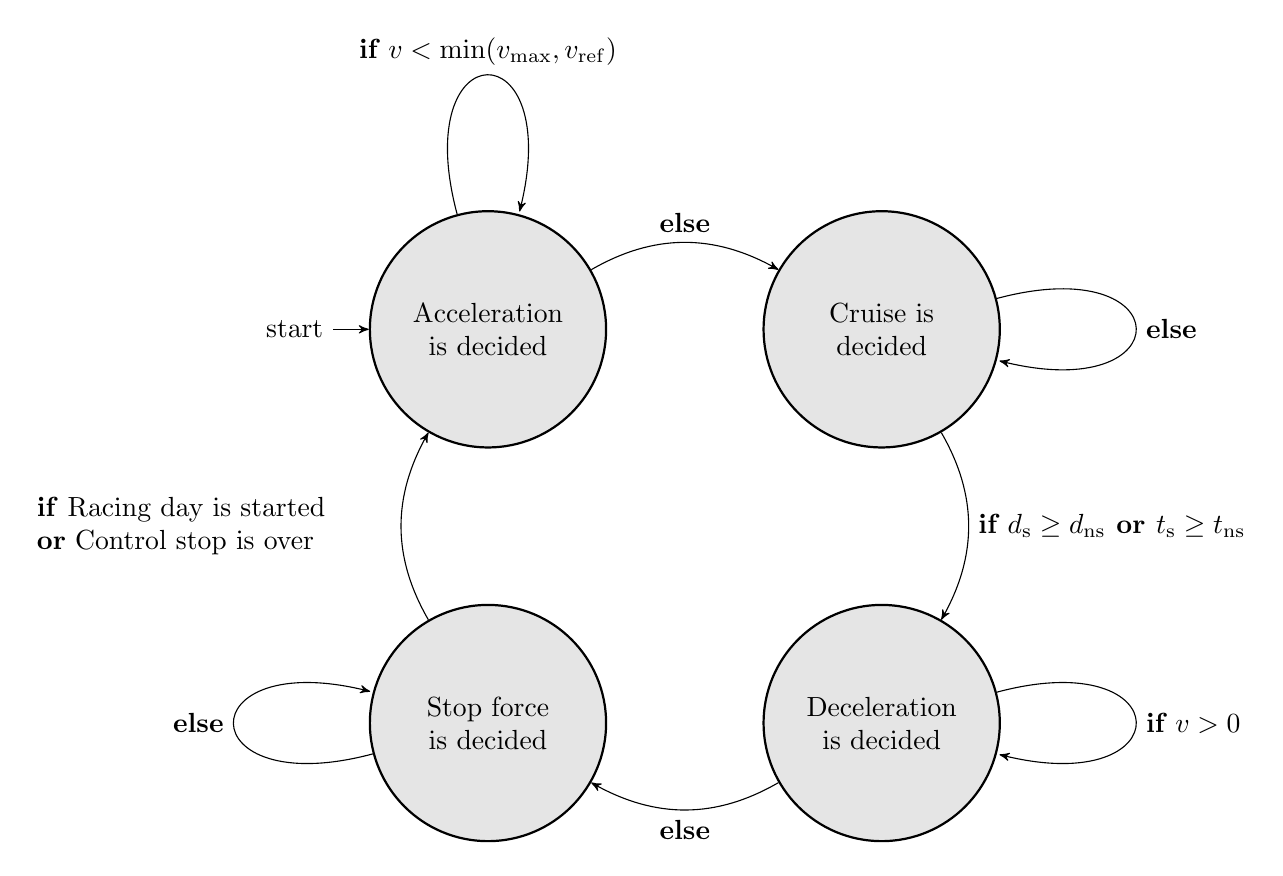
\begin{tikzpicture}[node distance=5cm, >=stealth',
	every state/.style={circle, minimum size=3cm, thick, draw=black, fill=gray!20!white}]
	\node[state, initial, text width=2 cm, align=center] (acc) {Acceleration is decided};
	\node[state] (cruise) [right of=acc, text width=2 cm, align=center] {Cruise is decided};
	\node[state] (dec) [below of=cruise, text width=2 cm, align=center] {Deceleration is decided};
	\node[state] (stop) [left of=dec, text width=2 cm, align=center] {Stop force is decided};
	\path[->] (acc) edge [loop above] node {$\textbf{if } v < \min(v_\mathrm{max}, v_\mathrm{ref})$} (acc);
	\path[->] (acc) edge [bend left] node[above] {\textbf{else}} (cruise);
	\path[->] (cruise) edge [loop right] node {\textbf{else}} (cruise);
	\path[->] (cruise) edge [bend left] node[right] {$\textbf{if } d_\mathrm{s} \geq d_\mathrm{ns} \textbf{ or } t_\mathrm{s} \geq t_\mathrm{ns}$} (dec);
	\path[->] (dec) edge [loop right] node {$\textbf{if } v > 0$} (dec);
	\path[->] (dec) edge [bend left] node[below] {\textbf{else}} (stop);
	\path[->] (stop) edge [loop left] node {\textbf{else}} (stop);
	\path[->] (stop) edge [bend left] node[left, text width=4.5 cm] {\textbf{if} \enquote{Racing day is started} \\ \textbf{or} \enquote{Control stop is over}} (acc);
\end{tikzpicture}
	\caption{Finite state machine of the Decision Maker with the four control modes.}
	\label{fig:simStateMachine}
\end{figure}
%\begin{algorithm}
%	\caption{Decision Maker pseudocode.}
%	\label{alg:decisionMaker}
%	\begin{algorithmic}
%	\Input{Training sentences $S_{i}$}
%	\Output{Sentence instances with cost-vectors for training $S_{i,c_i}$}
	\State Check if a control stop is approaching: $d_\mathrm{s} \geq d_\mathrm{ns}$
	\State Check if the end of the day is near: $t_\mathrm{s} \geq t_\mathrm{ns}$
	\State Check if the racing day is started
	\If{\enquote{Overnight stop is needed}}  \Comment{Deceleration}
	\If{$v > 0$}
	\State \enquote{Deceleration is decided} $\gets$ "true"
	\Else
	\State \enquote{Stop force is decided} $\gets$ "true"
	\EndIf
	\ElsIf{\enquote{Control stop is needed}}
	\If{$v > 0$}
	\State \enquote{Deceleration is decided} $\gets$ "true"
	\Else
	\State \enquote{Stop force is decided} $\gets$ "true"
	\If{30 minutes have passed}
	\State \enquote{Control stop is over} $\gets$ "true"
	\EndIf
	\EndIf
	\ElsIf{\enquote{Racing day is started}}  \Comment{Acceleration}
	\If{$v < 0.9 \cdot \min(v_\mathrm{max}, v_\mathrm{ref})$}
	\State \enquote{Acceleration is decided} $\gets$ "true"
	\Else
	\State \enquote{Cruise is decided} $\gets$ "true"
	\EndIf
	\ElsIf{\enquote{Control stop is over}}
	\If{$v < 0.9 \cdot \min(v_\mathrm{max}, v_\mathrm{ref})$}
	\State \enquote{Acceleration is decided} $\gets$ "true"
	\Else
	\State \enquote{Cruise is decided} $\gets$ "true"
	\EndIf
	\Else
	\State \enquote{Cruise is decided} $\gets$ "true"  \Comment{Cruise}
	\EndIf

\end{algorithmic}
%\end{algorithm}


\subsection{Controllers}
\label{sec:simDriverControllers}
In this \texttt{Subsystem}, human-like behavior is simulated using a combination of two PI controllers and one cascaded controller. The latter is primarily responsible for setting the cruising velocity, while the formers handle acceleration and deceleration.

In Simulink, the maximal step size is set to $\unit[0.2]{s}$ to prevent divergent behavior of the controllers. If the step size is set to a larger value, the controllers may become unstable.

Nine inputs are received and only one output is generated as listed in~\cref{tab:simInOutControllers}.
\begin{table}[htbp]
	\centering
	\caption{Input/Output signals for the Controllers.}
	\label{tab:simInOutControllers}
	
	\begin{tabular}{c l l l l}
		\toprule
		& Block & Signal & Symbol & Type \\ 
		\midrule
		\multirow{9}{*}{Input from}
		& Plant & SoC & $x_\mathrm{SoC}$ & Float \\
		& Plant & Traction force bounds & $F_\mathrm{trac,lim}$ & Float \\
		& Plant & Car velocity & $v$ & Float \\
		& Simulink & Absolute time & $t_\mathrm{sim}$ & Float \\
		& Plant & Driven distance & $d$ & Float \\
		& -- & Maximal speed & $v_\mathrm{max}$ & Float \\
		& Decision Maker & Acceleration is decided & Acc is dec & Binary \\
		& Decision Maker & Deceleration is decided & Dec is dec & Binary \\
		& Decision Maker & Cruise is decided & Cruise is dec & Binary \\
		\midrule
		\multirow{1}{*}{Output to}
		& Plant & Requested traction force & $F_\mathrm{trac,req}$ & Float \\
		\bottomrule
	\end{tabular}
\end{table}

\paragraph{Acceleration and Deceleration}
These two \texttt{Subsystems} are constructed in the same way, with the only exception of a positive or negative constant acceleration in the code, $a_\mathrm{acc}$ or $a_\mathrm{dec}$, respectively.

As soon as acceleration or deceleration is decided, time and car velocity values are stored in the memory. These parameters are used to generate the corresponding reference ramp velocity $v_\mathrm{ref}$ with constant slope. The difference between reference and actual velocity $v_\mathrm{ref} - v$ used as input to the \texttt{PID(s)} built-in block, where the traction force bounds ensure that the output requested traction force is limited and that the integral term does not saturate. For this purpose, the clamping anti-reset windup (ARW) is activated.

\paragraph{Cruise}
For the majority of the time, a more or less constant reference velocity $v_\mathrm{ref}$ has to be followed. Its value is estimated considering the current SoC value, as illustrated in~\cref{fig:simCascadedController}. This single input multiple output behavior is achieved with a cascaded controller, where the fast PI controller converts velocity in requested traction force, while the slow PI controller translates SoC values into velocity. In case a higher SoC than the reference is detected, the velocity is increased to consume the extra energy stored in the battery. The opposite is true for a lower SoC detection.
\begin{sidewaysfigure}[htbp]
	\centering
	% Styles
\tikzset{
	midBlock/.style = {rectangle, thick, minimum width=2cm, minimum height=2cm,text centered, text width=2cm, draw=black, fill=white},
	arrow/.style= {thick, black, ->, >=stealth},
	line/.style= {thick, black},
	textOutput/.style = {black,right},
	textInput/.style = {black,left},
	container/.style = {gray,dashed},
	sum/.style = {circle, minimum size=0.7cm, thick, draw=black, fill=white},
	%sum
	charge node/.style={inner sep=0pt},
	pics/sum block/.style n args={4}{
		code={
			\path node (n) [draw, circle, inner sep=0pt, minimum size=0.7cm] {}
			(n.north) +(0,-1.5mm) node [charge node] {$#1$}
			(n.south) +(0,1.5mm) node [charge node] {$#2$}
			(n.west) +(1.5mm,0) node [charge node] {$#3$}
			(n.east) +(-1.5mm,0) node [charge node] {$#4$}
			;
		}
	}
}
\begin{tikzpicture}
	% Definition
	%for three arrows
	\def\up{0.5}
	\def\down{-\up}
	\def\right{0.5}
	\def\left{-\right}
	%radius
	\def\radius{0.07}
	
	% Blocks
	\matrix[column sep=1.4cm, row sep=1cm]{
		%first row
		& & & \coordinate (c14); & &  \coordinate (c16); & & & &
		\\
		%second row
		\coordinate (c21); & \node[midBlock] (SoCref) {SoC$_\mathrm{ref}(d)$ \\ Estimator}; & \node[sum] (sumSoC) {}; & \node[midBlock] (Cslow) {PI$_\mathrm{slow}$}; & \node[sum] (sumVel) {}; &  \node[midBlock] (Cfast) {PI$_\mathrm{fast}$}; & \node[midBlock] (plant) {Plant}; & \coordinate (c28); & \coordinate (c29); &
		\\
		%third row
		& & & & \coordinate (c35); &  & & \coordinate (c38); & &
		\\
		%fourth row
		& & \coordinate (c43); & & &  & & \coordinate (c48); & &
		\\
	};
	
	% Arrows;
	%horizontal
	\draw[arrow] (c21) node[textInput] {$d$} -- (SoCref);
	\draw[arrow] (SoCref) -- (sumSoC) node[midway, above] {$x_\mathrm{SoC,ref}$};
	\draw[arrow] (sumSoC) -- (Cslow);
	\draw[arrow] (Cslow) -- (sumVel) node[midway, above] {$v_\mathrm{ref}$};
	\draw[arrow] (sumVel) -- (Cfast);
	\draw[arrow] (Cfast) -- (plant) node[midway, above] {$F_\mathrm{trac,req}$};
	\draw[arrow] ([yshift=\up cm]plant.east) -- ([yshift=\up cm]c29) node[textOutput] {$x_\mathrm{SoC}$};
	\draw[arrow] ([yshift=\down cm]plant.east) -- ([yshift=\down cm]c29) node[textOutput] {$v$};
	\draw[line] ([xshift=\left cm]c38) -- (c35);
	\draw[line] ([xshift=\right cm]c48) -- (c43);
	%vertical
	\draw[line] ([xshift=\left cm, yshift=\down cm]c28) -- ([xshift=\left cm]c38);
	\draw[line] ([xshift=\right cm, yshift=\up cm]c28) -- ([xshift=\right cm]c48);
	\draw[arrow] (c35) -- (sumVel);
	\draw[arrow] (c43) -- (sumSoC);
	\draw[arrow] (c16) node[textInput,above] {$F_\mathrm{trac,lim}$} -- (Cfast);
	\draw[arrow] ([xshift=\left cm]c14) node[textInput,above] {$v_\mathrm{up}$} -- ([xshift=\left cm]Cslow.north);
	\draw[arrow] ([xshift=\right cm]c14) node[textInput,above] {$v_\mathrm{lo}$} -- ([xshift=\right cm]Cslow.north);
	
	% Dots
	\fill [black] ([xshift=\left cm, yshift=\down cm]c28) circle (\radius cm);
	\fill [black] ([xshift=\right cm, yshift=\up cm]c28) circle (\radius cm);
	
	%sum
	\path pic at (sumSoC) {sum block={}{-}{+}{}};
	\path pic at (sumVel) {sum block={}{-}{+}{}};
	
\end{tikzpicture}
	\caption{Block diagram representation of the cascaded cruise controller.}
	\label{fig:simCascadedController}
\end{sidewaysfigure}

The slow controller receives two additional inputs that serve the purpose of limiting the velocity to appropriate values and activating the ARW.
\begin{align}
	v_\mathrm{up} &= \min (v_\mathrm{max}(d),v_\mathrm{cruise}) \\
	v_\mathrm{lo} &= \min (v_\mathrm{max}(d),v_\mathrm{cruise},v_\mathrm{min})
\end{align}
where $v_\mathrm{up}$ and $v_\mathrm{lo}$ are the upper and lower velocity bounds, $v_\mathrm{max}$ is the maximal speed limit, $v_\mathrm{min}$ is the minimal open road velocity, and $v_\mathrm{cruise}$ is the imposed maximal cruise velocity. The latter velocity is necessary to limit the maximum speed that our car can sustain. Their numerical values are listed in~\cref{tab:simParametersDriver}.
\begin{table}[htbp]
	\centering
	\caption{Modeling parameters for the Driver.}
	\label{tab:simParametersDriver}
	
	\begin{tabular}{l l r l}
		\toprule
		Parameter                       		& Symbol                & Value 	& Unit\\ 
		\midrule
		Maximal cruise velocity & $v_\mathrm{cruise}$ & 110 & \unitfrac{km}{h} \\
		Minimal open road velocity & $v_\mathrm{min}$ & 60 & \unitfrac{km}{h} \\
		Acceleration constant & $a_\mathrm{acc}$ & 0.7 & \unitfrac{m}{s$^2$} \\
		Deceleration constant & $a_\mathrm{dec}$ & -0.7 & \unitfrac{m}{s$^2$} \\
		\bottomrule
	\end{tabular}
\end{table}

\begin{table}[htbp]
	\centering
	\caption{Control parameters used in controllers of the Driver.}
	\label{tab:simParametersControllers}
	
	\begin{tabular}{l c c}
		\toprule
		& Proportional & Integral / $\unitfrac{1}{s}$ \\ 
		\midrule
		PI$_\mathrm{acc}$
		& 4000 & 80 \\
		\midrule
		PI$_\mathrm{dec}$
		& 4000 & 80 \\
		\midrule
		PI$_\mathrm{fast}$
		& 2000 & 500 \\
		\midrule
		PI$_\mathrm{slow}$
		& -1000 & 10 \\
		
		\bottomrule
	\end{tabular}
\end{table}


% !TeX spellcheck = en_US
% !TeX encoding = UTF-8
% !TeX root = ../report.tex

\chapter{Energy Usage Optimization and Long-Term Strategy}
\label{chp:strategy}
This chapter outlines the process for obtaining a realistic SoC reference profile for the cascaded cruise controller as a function of the driven distance. The goal is to minimize the driving time or, equivalently, optimize energy usage by ensuring that the energy spent exactly matches the energy budget at the end of the race. However, this method can result in solutions that do not respect the lower bound of the SoC throughout the race. To address this issue, a smaller constant mean velocity is determined such that the SoC trajectory exactly reaches the $x_\mathrm{SoC,min}$ at the point where the worst violation is detected.

Although this approach avoids the need for complex optimization algorithms, it presents several challenges due to the time/space nature of the problem. In fact, the SoC profile is shaped by the occurrence of recharging possibilities, namely during the overnight stops in time domain and control stops in space domain. Additionally, these stops sometimes overlap, further increasing the complexity. To address these challenges, the chapter is structured to first present the underlying idea with the help of an example that does not include control stops: Derivations in time domain are explained in~\cref{sec:strategyTimeDomain}, followed by the space domain in~\cref{sec:strategySpaceDomain}. Subsequently, practical consideration such as the possible intersection between the energies during an overnight stop, overlapping between control and overnight stops, and lower bound violations are explained in~\cref{sec:strategyPracticalConsideration}. Finally, a flow diagram representation of the recursive algorithm that connects the two domains and includes the aforementioned considerations is presented in~\cref{sec:strategyRecursiveAlgo}.
 

\section{General Concept}
As previously mentioned, the idea behind the strategy optimization is to ensure that the complete energy budget is used during the race. Mathematically, this can be expressed with the following expression:
\begin{equation}
	E_\mathrm{loss}(d_\mathrm{tot}) \overset{!}{=} E_\mathrm{budg}(d_\mathrm{tot}) \label{eq:strategyEgoalDtot}
\end{equation}
where $E_\mathrm{loss}$ is the energy loss function, $E_\mathrm{budg}$ is the energy budget function, and $d_\mathrm{tot}$ is total length of the race. To allow the detailed derivation of these two quantities in~\cref{sec:strategyTimeDomain}, a first conversion from space to time domain is needed. This is performed by assuming a constant mean velocity over the entire race:
\begin{equation}
	\overline{v}_\mathrm{tot} = \frac{d_\mathrm{tot}}{t_\mathrm{driv}} \label{eq:strategyMeanVelTot}
\end{equation}
where $t_\mathrm{driv}$ is the driving time, i.e., the time when the car is moving. Assuming a minimal driving time $t_\mathrm{driv}^*$ and an optimal mean velocity $\overline{v}_\mathrm{tot,opt}$,~\cref{eq:strategyEgoalDtot} can be reformulated to
\begin{equation}
	E_\mathrm{loss}(t_\mathrm{driv}^* \cdot \overline{v}_\mathrm{tot,opt}) \overset{!}{=} E_\mathrm{budg}(t_\mathrm{driv}^* \cdot \overline{v}_\mathrm{tot,opt}).
\end{equation}
This is graphically shown in~\cref{fig:strategyEintersectionUnitedStops} as an intersection of the two curves: in blue the energy loss and in black the energy budget. 
\begin{figure}[htbp]
	\centering
	\begin{externalize}{intersectionStrategy}
			% This file was created by matlab2tikz.
%
%The latest updates can be retrieved from
%  http://www.mathworks.com/matlabcentral/fileexchange/22022-matlab2tikz-matlab2tikz
%where you can also make suggestions and rate matlab2tikz.
%
%This file has been created via figure2tikz on 03-Jan-2023 22:14:09.
%
\begin{tikzpicture}

\begin{axis}[%
width=\textwidth,
height=0.3\textwidth,
unbounded coords=jump,
xmin=0,
xmax=40,
xlabel style={font=\color{white!15!black}},
xlabel={Driving time / h},
ymin=0,
ymax=40,
ylabel style={font=\color{white!15!black}},
ylabel={Energy / kWh},
axis background/.style={fill=white},
grid=both,
legend pos=north west,
legend cell align={left},
legend style={draw=none},
]
\addplot [color=black, thick]
  table[]{img/intersectionStrategy/intersectionStrategy-1.tsv};
  \addlegendentry{Energy budget}
\addplot [color=blue, thick]
  table[]{img/intersectionStrategy/intersectionStrategy-2.tsv};
  \addlegendentry{Energy loss}
\addplot [color=red, dashed, thick, forget plot]
  table[]{img/intersectionStrategy/intersectionStrategy-3.tsv};
\addplot [color=red, only marks, mark size=2pt, mark=*, mark options={solid, red}, forget plot]
  table[]{img/intersectionStrategy/intersectionStrategy-4.tsv};
\node[red, fill=white] at (axis cs: 32.5,5) {$t_\mathrm{driv}^*$};
\addplot [color=black, forget plot]
  table[]{img/intersectionStrategy/intersectionStrategy-5.tsv};
\end{axis}
\end{tikzpicture}%
		\end{externalize}
	\caption{Graphical representation of the intersection between the energy budget and energy loss as a function of driving time. The vertical lines represent the overnight stops.}
	\label{fig:strategyEintersection}
\end{figure}

After this step into time domain, the analysis of the energy content in the battery as a function of the driven distance can be performed in the space domain, as explained in~\cref{sec:strategySpaceDomain}.


\subsection{Time Domain}
\label{sec:strategyTimeDomain}
The energy budget and energy loss values are derived in the following paragraphs.

\paragraph{Energy Budget}
The available energy budget for the race is calculated by adding the energy generated by the solar panels and the energy stored in the battery. To ensure safety, the battery is not fully depleted during the race and is used within certain limits.
\begin{equation}
	E_\mathrm{budg}(t_\mathrm{driv}) = E_\mathrm{PV}(t_\mathrm{driv}) + E_\mathrm{bat,safe}. \label{eq:strategyEbudgetTotTime}
\end{equation}
The PV energy is the first contribution and is found as follows:
\begin{equation}
	E_\mathrm{PV} = \int \tilde{P}_\mathrm{PV}(t) \;\mathrm{d}t = \int A_\mathrm{PV} \cdot G(t) \cdot \eta_\mathrm{PV} \cdot \tilde{\eta}_\mathrm{CF} \cdot \eta_\mathrm{loss} \;\mathrm{d}t
\end{equation}
where $\tilde{\eta}_\mathrm{CF}$ is assumed constant with an estimated value of 0.979 by considering $\overline{T}_\mathrm{amb} = \unit[28]{\celsius}$ and $\overline{v}_\mathrm{eff} = \unitfrac[112]{km}{h}$ in~\cref{eq:modelingPVtempPV}.

The second contribution is the energy that the battery can provide and it is represented by a fraction of the total energy stored at the beginning of the race:
\begin{equation}
	E_\mathrm{bat,safe} = (x_\mathrm{SoC,max} - x_\mathrm{SoC,min}) \cdot E_\mathrm{bat,max}. \label{eq:strategyEbatSafe}
\end{equation}
\Cref{eq:strategyEbatSafe} assumes that the state of energy (SoE) is equal to the SoC by assuming a constant open-circuit voltage~\cite{fawidmer:2016mt}.
\begin{equation}
	x_\mathrm{SoE} = \frac{1}{E_\mathrm{bat,max}} \cdot \int_{Q_\mathrm{bat,max}}^{Q_\mathrm{bat}} U_\mathrm{bat,oc} \;\mathrm{d} Q_\mathrm{bat}^* = \frac{1}{Q_\mathrm{bat,max}} \cdot \int_{0}^{t} - \eta_\mathrm{c} \cdot I_\mathrm{bat}(t) \;\mathrm{d}t = x_\mathrm{SoC}. \label{eq:strategySoCequalSoE}
\end{equation}


\paragraph{Energy Loss}
During the race, the car loses energy due to inefficiency in the components, rolling friction between the wheels and the road, and aerodynamic friction with the surrounding air.
\begin{equation}
	E_\mathrm{loss} = E_\mathrm{ineff} + E_\mathrm{roll} + E_\mathrm{aero} \label{eq:strategyElossSum}
\end{equation}
To simplify this expression, the energy inefficiency $E_\mathrm{ineff}$ is summarized as a constant inefficiency parameter $\eta_\mathrm{ineff}$, which is explained in~\cref{eq:strategyInefficiency} to~\cref{eq:strategyBearForce} below. Therefore,~\cref{eq:strategyElossSum} can be rewritten as
\begin{align}
	E_\mathrm{loss} &= \frac{1}{\eta_\mathrm{ineff}} \cdot (E_\mathrm{roll} + E_\mathrm{aero}) \label{eq:strategyElossApproxIneff}\\
	&= \frac{1}{\eta_\mathrm{ineff}} \cdot (F_\mathrm{roll} \cdot d_\mathrm{tot} + F_\mathrm{aero} \cdot d_\mathrm{tot}) \\
	&= \frac{d_\mathrm{tot}}{\eta_\mathrm{ineff}} \cdot \left(c_\mathrm{roll} \cdot m_\mathrm{tot} \cdot g + \frac{1}{2} \cdot \rho_\mathrm{air} \cdot A_\mathrm{front} \cdot c_\mathrm{aero} \cdot \overline{v}_\mathrm{tot}^2 \right) \label{eq:strategyELossVel}
\end{align}
where $E_\mathrm{roll}$ is the energy loss due to rolling friction and $E_\mathrm{aero}$ is the energy loss due to aerodynamic friction.~\Cref{fig:inclination} shows that the inclination of the road is relative small. Hence, $F_\mathrm{roll}$ can be approximated as independent on time or distance:
\begin{equation}
	F_\mathrm{roll} = c_\mathrm{roll} \cdot m_\mathrm{tot} \cdot g \quad , \quad \text{if} \quad v \geq 0
\end{equation}

In order to calculate $\eta_\mathrm{ineff}$ as accurately as possible, its value is estimated using the results of a single day simulation. Combining~\cref{eq:strategyElossSum} with~\cref{eq:strategyElossApproxIneff} yields
\begin{equation}
	\eta_\mathrm{ineff} \approx \frac{\tilde{E}_\mathrm{roll} + \tilde{E}_\mathrm{aero}}{\tilde{E}_\mathrm{ineff} + \tilde{E}_\mathrm{roll} + \tilde{E}_\mathrm{aero}} \label{eq:strategyInefficiency}
\end{equation}
where the estimated energy loss due to inefficiency is obtained by considering the losses that occur in the motor, battery, and bearing:
\begin{equation}
	\tilde{E}_\mathrm{ineff} = \tilde{E}_\mathrm{mot,loss} + \tilde{E}_\mathrm{bat,loss} + \tilde{E}_\mathrm{bear}.
\end{equation}
All estimated energy contributions are obtained as follows:
\begin{align}
	\tilde{E}_\mathrm{roll} &= \int F_\mathrm{roll}(t_\mathrm{sim}) \cdot v(t_\mathrm{sim}) \;\mathrm{d}t_\mathrm{sim} \\
	\tilde{E}_\mathrm{aero} &= \int F_\mathrm{aero}(t_\mathrm{sim}) \cdot v(t_\mathrm{sim}) \;\mathrm{d}t_\mathrm{sim} \\
	\tilde{E}_\mathrm{mot,loss} &= \int P_\mathrm{mot,el}(t_\mathrm{sim}) - P_\mathrm{mot,mec}(t_\mathrm{sim}) \;\mathrm{d}t_\mathrm{sim} \\
	\tilde{E}_\mathrm{bat,loss} &= \int R_\mathrm{bat} \cdot I_\mathrm{bat}^2(t_\mathrm{sim}) \;\mathrm{d}t_\mathrm{sim} \\
	\tilde{E}_\mathrm{bear} &= F_\mathrm{bear} \cdot d_\mathrm{tot} \label{eq:strategyBearForce}
\end{align}
resulting in an approximated value of
\begin{equation}
	\eta_\mathrm{ineff} = 0.93.
\end{equation}
Therefore, inserting~\cref{eq:strategyMeanVelTot} in~\cref{eq:strategyELossVel} results in the equation of interest for the energy loss, where it becomes a function of the driving time only:
\begin{equation}
	E_\mathrm{loss}(t_\mathrm{driv}) = \frac{d_\mathrm{tot}}{\eta_\mathrm{ineff}} \cdot \left(c_\mathrm{roll} \cdot m_\mathrm{tot} \cdot g + \frac{1}{2} \cdot \rho_\mathrm{air} \cdot A_\mathrm{front} \cdot c_\mathrm{aero} \left(\frac{d_\mathrm{tot}}{t_\mathrm{driv}}\right)^2\right). \label{eq:strategyELossTime}
\end{equation}
Really small values of the driving time to finish the race corresponds to a high mean velocity, and subsequently, a high aerodynamic energy loss.

Therefore, the minimal driving time is finally determined by the intersection of the two energy functions just derived as shown in~\cref{fig:strategyEintersection}. As a result, the optimal average velocity is obtained:
\begin{equation}
	\overline{v}_\mathrm{tot,opt} = \frac{d_\mathrm{tot}}{t_\mathrm{driv}^*}. \label{eq:strategyOptMeanVelTot}
\end{equation}


\subsection{Space Domain}
\label{sec:strategySpaceDomain}
The objective in the spatial domain is to express the energy content of the battery in terms of distance, as depicted in~\cref{fig:strategyEbat}.
\begin{figure}[htbp]
	\centering
	\begin{externalize}{EbatStrategy}
		% This file was created by matlab2tikz.
%
%The latest updates can be retrieved from
%  http://www.mathworks.com/matlabcentral/fileexchange/22022-matlab2tikz-matlab2tikz
%where you can also make suggestions and rate matlab2tikz.
%
%This file has been created via figure2tikz on 10-Jan-2023 22:03:46.
%
\begin{tikzpicture}

\begin{axis}[%
width=\textwidth,
height=0.3\textwidth,
unbounded coords=jump,
xmin=0,
xmax=3000,
%xlabel style={font=\color{white!15!black}},
xtick={0,500,1000,1500,2000,2500,3000},
xticklabels={0,500,1000,1500,2000,2500,3000},
xlabel={Distance / km},
ymin=0,
ymax=5,
%ylabel style={font=\color{white!15!black}},
ytick={0,1,2,3,4,5},
yticklabels={0,1,2,3,4,5},
ylabel={Battery energy / kWh},
axis background/.style={fill=white},
grid=both,
]
\addplot [color=black, thick, forget plot]
  table[]{img/EbatStrategy/EbatStrategy-1.tsv};
\addplot [color=black, thick, forget plot]
  table[]{img/EbatStrategy/EbatStrategy-2.tsv};
\end{axis}
\end{tikzpicture}%
	\end{externalize}
	\caption{Simplified battery energy content where only the overnight stops are considered. The vertical lines represents the overnight stops.}
	\label{fig:strategyEbat}
\end{figure}

The equation for the SoC is obtained by dividing the battery energy by the maximum stored energy and utilizing~\cref{eq:strategySoCequalSoE}.
\begin{equation}
	x_\mathrm{SoC}(d) = x_\mathrm{SoE}(d) = \frac{E_\mathrm{bat}(d)}{E_\mathrm{bat,max}} 
\end{equation}

\paragraph{Battery Energy}
The energy content in the battery is found as a function of the driven distance
\begin{equation}
	E_\mathrm{bat}(d) = E_\mathrm{bat,max} + E_\mathrm{PV}(d) - E_\mathrm{loss}(d), \label{eq:strategyEbatDist}
\end{equation}
where the energy loss of~\cref{eq:strategyELossTime} can be rewritten as a function of distance by exploiting the optimal mean velocity found in~\cref{eq:strategyOptMeanVelTot}:
\begin{equation}
	E_\mathrm{loss}(d) = \frac{d}{\eta_\mathrm{ineff}} \cdot \left(c_\mathrm{roll} \cdot m_\mathrm{tot} \cdot g + \frac{1}{2} \cdot \rho_\mathrm{air} \cdot A_\mathrm{front} \cdot c_\mathrm{aero} \cdot \overline{v}_\mathrm{tot,opt}^2 \right)
\end{equation}

In all these calculations, the potential energy shown in~\cref{fig:potEnergy} is neglected because its values are small compared to the other energy contributions of~\cref{eq:strategyEbatDist}.
\begin{equation}
	E_\mathrm{pot}(d) = m_\mathrm{tot} \cdot g \cdot h(d)
\end{equation}
\begin{figure}[htbp]
	\centering
	\begin{externalize}{potEnergy}
		% This file was created by matlab2tikz.
%
%The latest updates can be retrieved from
%  http://www.mathworks.com/matlabcentral/fileexchange/22022-matlab2tikz-matlab2tikz
%where you can also make suggestions and rate matlab2tikz.
%
%This file has been created via figure2tikz on 03-Jan-2023 14:30:09.
%
\begin{tikzpicture}

\begin{axis}[%
width=\textwidth,
height=0.3\textwidth,
xmin=0,
xmax=3000,
%xlabel style={font=\color{white!15!black}},
xtick={0,500,1000,1500,2000,2500,3000},
xticklabels={0,500,1000,1500,2000,2500,3000},
xlabel={Distance / km},
ymin=0,
ymax=0.5,
%ylabel style={font=\color{white!15!black}},
ytick={0,0.1,0.2,0.3,0.4,0.5},
yticklabels={0,0.1,0.2,0.3,0.4,0.5},
ylabel={Potential energy / kWh},
axis background/.style={fill=white},
grid=both,
]
\addplot [black, thick, forget plot]
  table[]{img/potEnergy/potEnergy-1.tsv};
\end{axis}
\end{tikzpicture}%
	\end{externalize}
	\caption{Potential energy plotted as a function of distance.}
	\label{fig:potEnergy}
\end{figure}

\newpage
\section{Practical Considerations}
\label{sec:strategyPracticalConsideration}
This section addresses exceptional edge cases that must be considered in order to achieve accurate and practical outcomes.


\subsection{Intersection During Overnight Stop}
\label{sec:strategyIntDuringOvernight}
The first exceptional case to be taken into account is that the energy budget curve might intersect the energy loss curve during an overnight stop. In~\ref{fig:strategyEintersectionUnitedStopsError}, this occurrence happens at the end of the fourth day.
\begin{figure}[htbp]
	\centering
	\begin{externalize}{intersectionStrategyUnitedStopsError}
		% This file was created by matlab2tikz.
%
%The latest updates can be retrieved from
%  http://www.mathworks.com/matlabcentral/fileexchange/22022-matlab2tikz-matlab2tikz
%where you can also make suggestions and rate matlab2tikz.
%
%This file has been created via figure2tikz on 10-Jan-2023 18:31:39.
%
\begin{tikzpicture}

\begin{axis}[%
width=\textwidth,
height=0.3\textwidth,
unbounded coords=jump,
xmin=23,
xmax=34,
xlabel style={font=\color{white!15!black}},
xlabel={Driving time / h},
ymin=25,
ymax=35,
ylabel style={font=\color{white!15!black}},
ylabel={Energy / kWh},
axis background/.style={fill=white},
grid=both,
legend pos=north west,
legend cell align={left},
legend style={draw=none},
]
\addplot [color=black, thick]
  table[]{img/intersectionStrategyUnitedStopsError/intersectionStrategyUnitedStopsError-1.tsv};
  \addlegendentry{Energy budget}
\addplot [color=blue, thick]
  table[]{img/intersectionStrategyUnitedStopsError/intersectionStrategyUnitedStopsError-2.tsv};
  \addlegendentry{Energy loss}
\addplot [color=red, only marks, mark size=1.7pt, mark=*, mark options={solid, red}, forget plot]
  table[]{img/intersectionStrategyUnitedStopsError/intersectionStrategyUnitedStopsError-4.tsv};
\addplot [color=black, thick, forget plot]
  table[]{img/intersectionStrategyUnitedStopsError/intersectionStrategyUnitedStopsError-5.tsv};
\addplot [color=red, dashed, thick, forget plot]
  table[]{img/intersectionStrategyUnitedStopsError/intersectionStrategyUnitedStopsError-3.tsv};
\node[red, fill=white] at (axis cs: 30,26.5) {$t_\mathrm{driv}^*$};
\end{axis}
\end{tikzpicture}%
	\end{externalize}
	\caption{Graphical representation of the intersection between the energy budget and energy loss during an overnight stop. The vertical line represents the fourth overnight stop.}
	\label{fig:strategyEintersectionUnitedStopsError}
\end{figure}

In this scenario, the actual driving time to finish the race will exceed $t_\mathrm{driv}^*$, as some energy is required to drive the final kilometers without using energy that is below $x_\mathrm{SoC,min}$. The energy needed is determined by subtracting the energy budget at the start of the overnight stop from the value at the intersection, while the remaining energy in the battery is found by subtracting the value at the end of the overnight stop from the value at the intersection. Therefore, the velocity has to be decreased by following the explanations in~\cref{sec:strategyLBviolation} below. Additionally, it is possible that the race is completed with some energy still remaining in the battery, as the velocity cannot exceed $v_\mathrm{cruise}$. This type of velocity adjustments is explained in~\cref{sec:strategyEleft} below.


\subsection{Overlapping Stops}
\label{sec:strategyOverlapStops}
The second exceptional case must be considered to accurately account for control stops that occur after 16:30. As explained in~\cref{sec:bwscRules}, the official rules impose that the time of a control stop is not spent during the overnight stops, but recovered from 08:00 on the following day. For instance, if a team stops at 16:50, the next day it can start driving at 08:20. This becomes relevant once the optimal mean velocity is calculated and the control stop cuts can be performed in time domain, as explained in~\cref{sec:strategyRecursiveAlgo} below. 


\subsection{Lower Bound Violation}
\label{sec:strategyLBviolation}
A further example of an exceptional case is shown in~\cref{fig:strategySoC} as the SoC profile violates the lower bound around the third overnight stop.
\begin{figure}[htbp]
	\centering
	\begin{externalize}{SoCstrategy}
		% This file was created by matlab2tikz.
%
%The latest updates can be retrieved from
%  http://www.mathworks.com/matlabcentral/fileexchange/22022-matlab2tikz-matlab2tikz
%where you can also make suggestions and rate matlab2tikz.
%
%This file has been created via figure2tikz on 04-Jan-2023 19:38:06.
%
\begin{tikzpicture}

\begin{axis}[%
width=\textwidth,
height=0.3\textwidth,
unbounded coords=jump,
xmin=0,
xmax=3000,
%xlabel style={font=\color{white!15!black}},
xtick={0,500,1000,1500,2000,2500,3000},
xticklabels={0,500,1000,1500,2000,2500,3000},
xlabel={Distance / km},
ymin=0,
ymax=100,
%ylabel style={font=\color{white!15!black}},
ytick={0,20,40,60,80,100},
yticklabels={0,20,40,60,80,100},
ylabel={State of charge / \%},
axis background/.style={fill=white},
grid=both,
%legend pos=south west,
%legend cell align={left},
%legend style={draw=none},
]
\addplot [color=black, thick, forget plot]
  table[]{img/SoCstrategy/SoCstrategy-1.tsv};
\addplot [color=black, thick, forget plot]
  table[]{img/SoCstrategy/SoCstrategy-2.tsv};
\addplot[dashed, black, thick] coordinates {(-1,10) (3100,10)};
\node[black, fill=white] at (axis cs: 250,10) {$x_\mathrm{SoC,min}$};
\addplot [color=orange, only marks, mark size=1.7pt, mark=*, mark options={solid, orange}, forget plot]
  table[]{img/SoCstrategy/SoCstrategy-3.tsv};
\end{axis}
\end{tikzpicture}%
	\end{externalize}
	\caption{Simplified SoC profile where only the overnight stops are considered. The SoC at the end of the race is precisely equal to the lower bound. The vertical lines represents the overnight stops.}
	\label{fig:strategySoC}
\end{figure}

To address this problem, the average velocity must be reduced to decrease the energy loss caused by the aerodynamic friction. The new average velocity should ensure that the energy budget is equivalent to the energy loss at the point of the worst violation, i.e., in the evening of the third day in this example. This can be mathematically represented by the following energy balance equation:
\begin{align}
	E_\mathrm{budg,det} &\overset{!}{=} E_\mathrm{loss,det}(\overline{v}_\mathrm{det}) \\
	E_\mathrm{PV,det} + E_\mathrm{bat,safe} &\overset{!}{=} \frac{\overline{v}_\mathrm{det} \cdot t_\mathrm{driv,det}}{\eta_\mathrm{ineff}} \cdot \left(c_\mathrm{roll} \cdot m_\mathrm{tot} \cdot g + \frac{1}{2} \cdot \rho_\mathrm{air} \cdot A_\mathrm{front} \cdot c_\mathrm{aero} \cdot \overline{v}_\mathrm{det}^2 \right) \label{eq:strategyEbalanceDetection}
\end{align}
where $\overline{v}_\mathrm{det}$ is the new mean velocity that guarantees that the $x_\mathrm{SoC,min}$ is respected where the worst violation is detected, as illustrated in~\cref{fig:strategySoCsafe}, and $t_\mathrm{driv,det}$ is the driving time until this violation. It is assumed that the worst violations can only occur at 17:00 of each day.
\begin{figure}[htbp]
	\centering
	\begin{externalize}{SoCsafeStrategy}
		\input{img/SoCsafeStrategy/SoCsafeStrategy.tex}
	\end{externalize}
	\caption{Simplified SoC profile where only the overnight stops are considered. The SoC where the worst detection occurs is precisely equal to the lower bound. The vertical lines represents the overnight stops.}
	\label{fig:strategySoCsafe}
\end{figure}

The PV energy until detection is calculated as follows:
\begin{equation}
	E_\mathrm{PV,det} = \int_{0}^{t_\mathrm{driv,det}} \tilde{P}_\mathrm{PV}(t) \;\mathrm{d}t = \int_{0}^{t_\mathrm{driv,det}} A_\mathrm{PV} \cdot G(t) \cdot \eta_\mathrm{PV} \cdot \tilde{\eta}_\mathrm{CF} \cdot \eta_\mathrm{loss} \;\mathrm{d}t.
\end{equation}
To better analyze~\cref{eq:strategyEbalanceDetection}, it can be rewritten as a third order polynomial:
\begin{equation}
	\overline{v}_\mathrm{det}^3 + \underbrace{\frac{c_\mathrm{roll} \cdot m_\mathrm{tot} \cdot g}{\frac{1}{2} \cdot \rho_\mathrm{air} \cdot A_\mathrm{front} \cdot c_\mathrm{aero}}}_{p} \cdot \overline{v}_\mathrm{det} + \underbrace{\frac{- \frac{\eta_\mathrm{ineff}}{t_\mathrm{det}} \cdot \left(E_\mathrm{PV,det} + E_\mathrm{bat,safe} \right)}{\frac{1}{2} \cdot \rho_\mathrm{air} \cdot A_\mathrm{front} \cdot c_\mathrm{aero}}}_{q} = 0. \label{eq:strategy3poly}
\end{equation}
The three possible solutions of~\cref{eq:strategy3poly} are investigated by considering the following relation between the coefficients $p$ and $q$, as explained in~\cite{wikipediaCardano:2022webpage}:
\begin{equation}
	\Delta = \frac{q^2}{4} + \frac{p^3}{27} \quad
	\begin{cases}
		> 0 \qquad & \Rightarrow \quad \text{1 real and 2 complex solutions}, \\
		< 0 \qquad & \Rightarrow \quad \text{3 real solutions}.
	\end{cases}
\end{equation}
The first case is always true, in fact $p > 0$ and $q^2 > 0$. Therefore, Cardano's equation can be used to find the single real solution:
\begin{equation}
	\overline{v}_\mathrm{det} = \sqrt[3]{u_1} +  \sqrt[3]{u_2}
\end{equation}
with
\begin{equation}
	u_1 = - \frac{q}{2} + \sqrt{\Delta} \qquad \text{and} \qquad u_2 = - \frac{q}{2} - \sqrt{\Delta}.
\end{equation}
To ensure that more energy is stored in the battery, its value must be smaller than the optimal velocity:
\begin{equation}
	\overline{v}_\mathrm{det} < \overline{v}_\mathrm{tot,opt}.
\end{equation}


\subsection{Energy Optimization After Corrected Worst Violation}
\label{sec:strategyEleft}
The final strategy discussed in~\ref{sec:strategyLBviolation} ensures that the $x_\mathrm{SoC,min}$ is met exactly at the position of the worst violation by decreasing the average velocity. However, after implementing this strategy, the car will have some remaining energy in the battery at the end of the race. Similarly, the first scenario presented in~\ref{sec:strategyIntDuringOvernight} also has this outcome. Therefore, it is possible to apply the same logic used in~\ref{sec:strategyTimeDomain} to determine the optimal average velocity that balances the energy usage between the corrected violation and the end of the race. Therefore, the energy balance equation is as follows:
\begin{equation}
	E_{\mathrm{budg,det,end}} \overset{!}{=} E_{\mathrm{loss,det,end}}(t_\mathrm{driv}). \label{eq:strategyEgoalDetEnd}
\end{equation}
The energy loss as function of the driving time is found as
\begin{equation}
	E_{\mathrm{loss,det,end}} = \frac{d_\mathrm{tot} - d_\mathrm{det}}{\eta_\mathrm{ineff}} \cdot \left(c_\mathrm{roll} \cdot m_\mathrm{tot} \cdot g + \frac{1}{2} \cdot \rho_\mathrm{air} \cdot A_\mathrm{front} \cdot c_\mathrm{aero} \left(\frac{d_\mathrm{tot} - d_\mathrm{det}}{t_\mathrm{driv} - t_\mathrm{driv,det}} \right)^2 \right),
\end{equation}
where $d_\mathrm{det}$ is the distance traveled until the corrected worst detection and similarly, $t_\mathrm{driv,det}$ is the driving time until the corrected worst detection. The two contributions of the energy budget are represented by the following equations:
\begin{align}
	E_\mathrm{PV,det,end} &= \int_{t_\mathrm{driv,det}}^{t_\mathrm{end}} \tilde{P}_\mathrm{PV}(t) \;\mathrm{d}t = \int_{t_\mathrm{driv,det}}^{t_\mathrm{end}} A_\mathrm{PV} \cdot G(t) \cdot \eta_\mathrm{PV} \cdot \tilde{\eta}_\mathrm{CF} \cdot \eta_\mathrm{loss} \;\mathrm{d}t, \\
	E_\mathrm{bat,safe,det} &= (x_\mathrm{SoC,det} - x_\mathrm{SoC,min}) \cdot E_\mathrm{bat,max}.
\end{align}
By exploiting the intersection between the two new curves, is it possible to find the optimal driving time between violation and finish line where~\cref{eq:strategyEgoalDetEnd} is satisfied. Therefore, the mean velocity of this segment is as follows:
\begin{equation}
	\overline{v}_\mathrm{det,end} = \frac{d_\mathrm{tot} - d_\mathrm{det}}{t_\mathrm{driv,end}^* - t_\mathrm{driv,det}}.
\end{equation}
This velocity cannot exceed the maximal cruise velocity:
\begin{equation}
	\overline{v}_\mathrm{det,end} \leq v_\mathrm{cruise}.
\end{equation}

Due to time constraints, this part is not going to be integrated in the final code. Nevertheless, the recursive algorithm explained in the following section takes this scenario into consideration.
%Control stops:
%\begin{equation}
%	d_{\mathrm{cs},j} \quad t_{\mathrm{driv,cs},j} \qquad j = 1, 2, ... , 9
%\end{equation}
%Overnight stops:
%\begin{equation}
%	t_{\mathrm{driv,os},k} \quad d_{\mathrm{os},k} \qquad k = 1, 2, ...
%\end{equation}

\newpage
\section{Recursive Algorithm}
\label{sec:strategyRecursiveAlgo}
In this section, a recursive algorithm that generates the reference SoC profile is presented. It incorporates all previously mentioned scenarios and includes the nine control stops that were omitted in earlier examples. The description follows the flow diagram shown in~\cref{fig:recursiveAlgorithm}.

The algorithm starts by calling the Velocity Finder function with the initial set of variables. The optimal mean velocity $\overline{v}_\mathrm{tot,opt}$ is calculated, as described in detail in~\cref{sec:strategyTimeDomain}. The only difference is that in this case, the control stops are taken into account. Specifically, the total time spent at control stops is subtracted from the overall driving time at the start of the race, as graphically shown in~\cref{fig:strategyEintersectionUnitedStops}. This adjustment is necessary because the energy loss function depends on the driving time, rather than the timing of the stops. Thus, it is crucial to consider these nine stops before the intersection.
\begin{figure}[htbp]
	\centering
	\begin{externalize}{intersectionStrategyUnitedStops}
		% This file was created by matlab2tikz.
%
%The latest updates can be retrieved from
%  http://www.mathworks.com/matlabcentral/fileexchange/22022-matlab2tikz-matlab2tikz
%where you can also make suggestions and rate matlab2tikz.
%
%This file has been created via figure2tikz on 09-Jan-2023 16:35:51.
%
\begin{tikzpicture}

\begin{axis}[%
width=\textwidth,
height=0.3\textwidth,
unbounded coords=jump,
xmin=0,
xmax=35,
xlabel style={font=\color{white!15!black}},
xlabel={Driving time / h},
ymin=0,
ymax=40,
ylabel style={font=\color{white!15!black}},
ylabel={Energy / kWh},
axis background/.style={fill=white},
grid=both,
legend pos=north west,
legend cell align={left},
legend style={draw=none},
]
\addplot [color=black, thick]
  table[]{img/intersectionStrategyUnitedStops/intersectionStrategyUnitedStops-1.tsv};
  \addlegendentry{Energy budget}
\addplot [color=blue, thick]
  table[]{img/intersectionStrategyUnitedStops/intersectionStrategyUnitedStops-2.tsv};
  \addlegendentry{Energy loss}
\addplot [color=red, dashed, thick, forget plot]
  table[]{img/intersectionStrategyUnitedStops/intersectionStrategyUnitedStops-3.tsv};
\addplot [color=red, only marks, mark size=2pt, mark=*, mark options={solid, red}, forget plot]
  table[]{img/intersectionStrategyUnitedStops/intersectionStrategyUnitedStops-4.tsv};
\addplot [color=black, thick, forget plot]
  table[]{img/intersectionStrategyUnitedStops/intersectionStrategyUnitedStops-5.tsv};
\node[red, fill=white] at (axis cs: 30,5) {$t_\mathrm{driv}^*$};
\end{axis}
\end{tikzpicture}%
	\end{externalize}
	\caption{Graphical representation of the intersection between the energy budget and energy loss as a function of driving time. The vertical lines represent the overnight stops, while the nine control stops are accounted for at the beginning of the race.}
	\label{fig:strategyEintersectionUnitedStops}
\end{figure}

At this point, the exceptional case mentioned in~\cref{sec:strategyIntDuringOvernight} could occur.

Once the optimal mean velocity is determined, the control stop positions can be converted to time. This enables the Overlaps Corrector to make adjustments for the scenario outlined in~\cref{sec:strategyOverlapStops}. Furthermore, the equations in the space domain are calculated as explained in~\cref{sec:strategySpaceDomain}.

Afterwards, the Violation Detector checks whether all SoC values meet the lower bound.
\begin{itemize}
	\item If any violation is identified, the problem is divided at the point of worst violation: The left portion in~\cref{fig:recursiveAlgorithm} is resolved using the methods outlined in~\cref{sec:strategyLBviolation} with the goal of matching the SoC of the worst violation with $x_\mathrm{SoC,min}$, while the right portion is solved using the equations in~\cref{sec:strategyEleft} with the goal of finding the mean velocity that ensures all available energy is used. The recursion is necessary because all possible violations must be individually addressed. After both the left and right loops are completed, the resulting signals must be concatenated to form the final results.
	\item On the other hand, if no violation is detected, the SoC Generator is called and the reference SoC profile is finally generated.
\end{itemize}

\begin{figure}[htbp]
	\centering
	\begin{externalize}{recursiveAlgorithm}
		% Styles
\tikzstyle{variables} = [rectangle, rounded corners, text centered, text width=3.8cm, draw=black, fill=white]
\tikzstyle{function} = [rectangle, minimum width=4cm, minimum height=1.5cm, text centered, text width=4cm, draw=black, fill=gray!20!white]
\tikzstyle{decision} = [diamond, aspect=2, inner xsep=0mm, text centered, text width=2cm, draw=black, fill=white]
\tikzstyle{arrow} = [thick,->,>=stealth]
	
\begin{tikzpicture}[node distance=2.5cm]
	% Definition
	\def\right{3}
	\def\left{-\right}
	\def\Nright{1.5}
	\def\Nleft{-\right}
	
	% Blocks
	\node (start) [] {};
	\node (inputVar) [variables, below of=start] {$d_\mathrm{start} = 0$ \\ $t_\mathrm{start} = 0$ \\ $x_\mathrm{SoC,start} = x_\mathrm{SoC,max}$ \\ $d_\mathrm{target} = d_\mathrm{tot}$ \\ $t_\mathrm{target} = \mathrm{NaN}$};
	\node (velFinder) [function, below of=inputVar] {Velocity Finder};
	\node (zero2detVar) [variables, left of=velFinder, xshift=\left cm] {$d_\mathrm{start} = 0$ \\ $t_\mathrm{start} = 0$ \\ $x_\mathrm{SoC,start} = x_\mathrm{SoC,max}$ \\ $d_\mathrm{target} = \mathrm{NaN}$ \\ $t_\mathrm{target} = t_\mathrm{driv,det}$};
	\node (det2endVar) [variables, right of=velFinder, xshift=\right cm] {$d_\mathrm{start} = d_\mathrm{det}$ \\ $t_\mathrm{start} = t_\mathrm{driv,det}$ \\ $x_\mathrm{SoC,start} = x_\mathrm{SoC,det}$ \\ $d_\mathrm{target} = d_\mathrm{tot}$ \\ $t_\mathrm{target} = \mathrm{NaN}$};
	\node (overCorr) [function, below of=velFinder] {Overlaps Corrector};
	\node (violDet) [function, below of=overCorr] {Violation Detector};
	\node (violIsDet) [decision, below of=violDet] {Violation \\ is detected?};
	\node (worstDetFinder) [function, below of=violIsDet] {Worst Violation Finder};
	\node (SoCgen) [function, below of=worstDetFinder] {SoC Generator};
	\node (SoCref) [below of=SoCgen] {};
	
	% Arrows
	\draw [arrow] (start) node[above] {start} -- (inputVar);
	\draw [arrow] (inputVar) -- (velFinder);
	\draw [arrow] (zero2detVar) -- (velFinder);
	\draw [arrow] (det2endVar) -- (velFinder);
	\draw [arrow] (velFinder) -- (overCorr);
	\draw [arrow] (overCorr) -- (violDet);
	\draw [arrow] (violDet) -- (violIsDet);
	\draw [arrow] (violIsDet) -- node[anchor=west] {yes} (worstDetFinder);
	\draw [arrow] (violIsDet.east) to["no" '] + (1,0) |-  (SoCgen.east);
	\draw [arrow] (worstDetFinder) -| (zero2detVar) node[midway, below, text width=3cm] {1. Solve left part \\ until violation};
	\draw [arrow] (worstDetFinder) -| (det2endVar) node[midway, below, text width=3cm] {2. Solve right part \\ after violation};
	\draw [arrow] (SoCgen) -- (SoCref) node[below] {$x_\mathrm{SoC,ref}$};
\end{tikzpicture}
	\end{externalize}
	\caption{Flow diagram of the recursive algorithm. Gray rectangles represent functions, rounded-corner rectangle set of variables, and the white rectangle a binary variable.}
	\label{fig:recursiveAlgorithm}
\end{figure}


% !TeX spellcheck = en_US
% !TeX encoding = UTF-8
% !TeX root = ../report.tex

\chapter{Results and Discussion}
\label{chp:results}
In this chapter, a detailed analysis of the driver's behavioral decision-making is presented in~\cref{sec:resultsDriverBehavior}. Additionally, through the Simulink simulation, a comprehensive sensitivity analysis of several key design parameters is conducted in~\cref{sec:resultsSensitivityAnalysis} to examine their impact on the total racing time. Lastly, in~\cref{sec:resultsStrategy}, the SoC profile that minimizes the driving time is shown and discussed.


\section{Simulation}
\subsection{Driver Behavior}
\label{sec:resultsDriverBehavior}
The first simulation results show how the driver's decisions affect the solar car's performance.~\Cref{fig:resultsDriverBehavior} consists of two plots, one displaying the car's velocity and the other showing the battery's SoC during the first $\unit[4]{hours}$ of the simulation. The reason for including these two quantities is that they are closely related through the cascaded cruise controller, as explained in~\cref{sec:simDriverControllers}. It is worth noting that the reference state of charge used to produce these results is not the optimal one determined by the method outlined in~\ref{chp:strategy}, but rather a simplified linear reference.
\begin{sidewaysfigure}[htbp]
	\centering
	\begin{externalize}{resultsDriverBehavior}
		\begin{tikzpicture}
	
	\begin{groupplot}[
		group style={
			group size=1 by 2,
			vertical sep=0.4cm,
			xlabels at=edge bottom,
			xticklabels at=edge bottom,
		},
		width=\textwidth,
		height=0.3\textwidth,
		unbounded coords=jump,
		xmin=0,
		xmax=4,
		grid=both,
		legend pos={south west},
		legend cell align={left},
		legend style={draw=none},
		]
		
		\nextgroupplot[
		xlabel near ticks,
		xtick={0,0.5,1,1.5,2,2.5,3,3.5,4},
		ylabel near ticks,
		ymin=0,
		ymax=120,
		ytick={0,20,40,60,80,100,120},
		yticklabels={0,20,40,60,80,100,120},
		ylabel={Velocity / $\unitfrac{km}{h}$},
		]
		\addplot [black, thick, dashdotdotted]
		table[]{img/resultsDriverBehaviorVel/resultsDriverBehaviorVel-1.tsv};
		\addlegendentry{$v_\mathrm{max}$}
		
		\addplot [black, dashed, thick]
		table[]{img/resultsDriverBehaviorVel/resultsDriverBehaviorVel-2.tsv};
		\addlegendentry{$v_\mathrm{cruise}$}
		
		\addplot [black, dashdotted, thick]
		table[]{img/resultsDriverBehaviorVel/resultsDriverBehaviorVel-3.tsv};
		\addlegendentry{$v_\mathrm{min}$}
		
		\addplot [blue, thick]
		table[]{img/resultsDriverBehaviorVel/resultsDriverBehaviorVel-4.tsv};
		\addlegendentry{$v_\mathrm{ref}$}
		
		\addplot [magenta, dashed, thick]
		table[]{img/resultsDriverBehaviorVel/resultsDriverBehaviorVel-5.tsv};
		\addlegendentry{$v$}
		
		\nextgroupplot[
		xlabel near ticks,
		xtick={0,0.5,1,1.5,2,2.5,3,3.5,4},
%		xticklabels={0,0.5,1,1.5,2,2.5,3,3.5,4},
		xlabel={Simulation time / h},
		ylabel near ticks,
		ymin=0,
		ymax=1.1,
		ytick={0,0.2,0.4,0.6,0.8,1},
		yticklabels={0,0.2,0.4,0.6,0.8,1},
		ylabel style={align=left}, ylabel=State of charge / --\\Control modes / --,
		]
		\addplot [green, thick]
		table[]{img/resultsDriverBehaviorSoC/resultsDriverBehaviorSoC-1.tsv};
		\addlegendentry{Stop force is decided}
		
		\addplot [red, thick]
		table[]{img/resultsDriverBehaviorSoC/resultsDriverBehaviorSoC-2.tsv};
		\addlegendentry{Cruise is decided}
		
		\addplot [cyan, thick]
		table[]{img/resultsDriverBehaviorSoC/resultsDriverBehaviorSoC-3.tsv};
		\addlegendentry{Deceleration is decided}
		
		\addplot [brown, thick]
		table[]{img/resultsDriverBehaviorSoC/resultsDriverBehaviorSoC-4.tsv};
		\addlegendentry{Acceleration is decided}
		
		\addplot [blue, thick]
		table[]{img/resultsDriverBehaviorSoC/resultsDriverBehaviorSoC-5.tsv};
		\addlegendentry{$x_\mathrm{SoC,ref}$}
		
		\addplot [magenta, dashed, thick]
		table[]{img/resultsDriverBehaviorSoC/resultsDriverBehaviorSoC-6.tsv};
		\addlegendentry{$x_\mathrm{SoC}$}
		
	\end{groupplot}
	
\end{tikzpicture}%
	\end{externalize}
	\caption{Group plot of the first simulated four hours of the race. Above, the velocity plot including all limits, the reference velocity in blue, and the car velocity in pink. Below, the SoC and control mode plot with reference SoC and SoC.}
	\label{fig:resultsDriverBehavior}
\end{sidewaysfigure}

The simulation begins with the \enquote{Acceleration is decided} mode active until the car reaches the target reference velocity. At this point, the \enquote{Cruise is decided} mode is engaged for several hours. The plots demonstrate that the car's velocity and SoC closely follow their respective references, thereby confirming the effectiveness of the cascaded controller. Additionally, the car's velocity stays within the expected range from $\unitfrac[60]{km}{h}$ to $\unitfrac[110]{km}{h}$. There is a slight deviation of the SoC from the reference at around $\unit[2.5]{hours}$ into the simulation, which can be attributed to the peak solar irradiance and the car's maximum velocity.

At around $\unit[3.4]{hours}$, the \enquote{Deceleration is decided} mode is activated as a control stop approaches. The car's velocity decreases until it comes to a stop, followed by the engaging of the mechanical brake through the activation of \enquote{Stop force is decided}. After $\unit[30]{minutes}$, the \enquote{Acceleration is decided} mode is activated again and the car gains speed until the target reference velocity is reached, at which point the \enquote{Cruise is decided} mode is engaged once more. During control stops, the car's velocity is zero but the SoC increases, highlighting the benefits of these safety check-points as opportunities to recharge the battery.

Overall, the driver demonstrates excellent tracking capabilities and makes appropriate decisions throughout the simulation.


\subsection{Sensitivity Analysis}
\label{sec:resultsSensitivityAnalysis}
The second results obtained with the simulation is the sensitivity analysis of various crucial design parameters. The goal is to determine the extent to which each car parameter affects the overall racing time when it is increased by 1\% with respect to its actual value used in~\cref{chp:modeling}. Mathematically, this can be represented by the following relation:
\begin{equation}
	\frac{\partial f}{\partial z_n} \approx \frac{\Delta t_\mathrm{sim,tot}}{\Delta z_n}
\end{equation}
where $f$ is the function represented by the simulation as explained below in~\cref{eq:resultsSimFctTime}, $z_n$ is the n-th parameter, and $t_\mathrm{sim,tot}$ is the simulated time to complete the race. As previously mentioned in~\cref{chp:simulation}, the time period from sunset until sunrise is not simulated. Additionally, the local partial derivative is approximated by 1\% increase of the n parameters:
\begin{equation}
	\Delta z_n = 0.01 \cdot z_n \quad , \quad n \in \{1,...,12\}.
\end{equation}
Lastly, the simulation can be thought of as a function of the twelve design parameters of interest that outputs the simulated time:
\begin{equation}
	f(c_\mathrm{aero}, A_\mathrm{front}, ...) = t_\mathrm{sim,tot} \label{eq:resultsSimFctTime}
\end{equation}
and that the increase in racing time is found as
\begin{equation}
	\Delta t_\mathrm{sim,tot} = t_{\mathrm{sim,tot,}n} - t_\mathrm{sim,tot}
\end{equation}
where $t_{\mathrm{sim,tot,}n}$ is simulated time to finish the race when the n-th parameter is increased, and $t_\mathrm{sim,tot}$ is the base case where all parameters are as presented in~\cref{chp:modeling}.

\Cref{fig:resultsSensitivityAnalysis} illustrates the results of the sensitivity analysis conducted as previously described.
\begin{figure}[htbp]
	\centering
	\begin{externalize}{sensitivityAnalysis}
		% This file was created by matlab2tikz.
%
%The latest updates can be retrieved from
%  http://www.mathworks.com/matlabcentral/fileexchange/22022-matlab2tikz-matlab2tikz
%where you can also make suggestions and rate matlab2tikz.
%
%This file has been created via figure2tikz on 19-Dec-2022 17:23:11.
%
\begin{tikzpicture}

\begin{axis}[%
width=0.9\textwidth,
height=0.5\textwidth,
%bar shift auto,
xmin=-6.5,
xmax=6.5,
xlabel style={font=\color{white!15!black}},
xlabel={Racing time increase / min},
ymin=-0.2,
ymax=11.2,
ytick={1,2,3,4,5,6,7,8,9,10},
yticklabels={{$e_\mathrm{mot}$},{$\eta_\mathrm{PV}$},{$Q_\mathrm{bat,max}$},{$r_\mathrm{w}$},{$U_\mathrm{bat,oc}$},{$R_\mathrm{bat}$},{$P_0$},{$c_\mathrm{roll}$},{$m_\mathrm{tot}$},{$c_\mathrm{aero}$, $A_\mathrm{front}$, $\rho_\mathrm{air}$}},
axis background/.style={fill=white},
grid=both,
]
\addplot[xbar, bar width=0.6, fill=white!30!orange, draw=black, area legend, 
nodes near coords,
node near coord style={fill=white, fill opacity=1},
] table[] {img/sensitivityAnalysis/sensitivityAnalysis-1.tsv};
%\addplot[forget plot, color=white!15!black] table[] {img/sensitivityAnalysis/sensitivityAnalysis-2.tsv};
\end{axis}
\end{tikzpicture}%
	\end{externalize}
	\caption{Results of the sensitivity analysis obtained by increasing the values of the variables used in~\cref{chp:modeling} by 1\%.}
	\label{fig:resultsSensitivityAnalysis}
\end{figure}

The plot clearly shows that the three aerodynamic parameters have the most significant contribution, represented by the same bar because they have the same impact. The second most influential factors are the motor and PV efficiency. The increase in the total mass, rolling friction coefficient and maximal battery capacity show similar absolute racing time increase. The wheel radius and the motor idle losses in the Willans model also have a notable impact.

The influence of the battery resistance and open-circuit voltage is so small that no clear trend can be observed. In fact, their impact on the total duration of the race is minimal.

It is important to note that this analysis is based on a 1\% increase in the current value of the parameters to enable a comparison, regardless of whether this change is truly applicable. Nevertheless, this analysis provides quantitative results that can be used to prioritize time and effort on areas that have the greatest potential to improve race outcomes.

In general, this analysis can be conducted also by considering different weather conditions and driver parameters:
\begin{equation}
	f(\text{car parameters, weather data, driver coefficients}) = t_\mathrm{sim,tot}.
\end{equation}


\section{Optimized State-of-Charge Reference Profile}
\label{sec:resultsStrategy}
In this section, the SoC reference profile generated with the approach thoroughly explained in~\cref{chp:strategy} is presented and discussed.~\Cref{fig:resultsSoCref} shows the resulting SoC trajectory as a function of distance when both overnight and control stops are taken into account.
\begin{figure}[htbp]
	\centering
	\begin{externalize}{resultsSoCsafe}
		% This file was created by matlab2tikz.
%
%The latest updates can be retrieved from
%  http://www.mathworks.com/matlabcentral/fileexchange/22022-matlab2tikz-matlab2tikz
%where you can also make suggestions and rate matlab2tikz.
%
%This file has been created via figure2tikz on 11-Jan-2023 11:34:24.
%
\begin{tikzpicture}

\begin{axis}[%
width=\textwidth,
height=0.5\textwidth,
unbounded coords=jump,
xmin=0,
xmax=3027.23523240565,
%xlabel style={font=\color{white!15!black}},
xtick={0,500,1000,1500,2000,2500,3000},
xticklabels={0,500,1000,1500,2000,2500,3000},
xlabel={Distance / km},
ymin=0,
ymax=100,
%ylabel style={font=\color{white!15!black}},
ytick={0,20,40,60,80,100},
yticklabels={0,20,40,60,80,100},
ylabel={State of charge / \%},
axis background/.style={fill=white},
grid=both,
legend pos=north east,
legend cell align={left},
legend style={draw=none},
]
\addplot [blue, dashdotted, thick]
  table[]{img/resultsSoCsafe/resultsSoCsafe-1.tsv};
  \addlegendentry{First iteration}
\addplot [blue, thick]
  table[]{img/resultsSoCsafe/resultsSoCsafe-2.tsv};
  \addlegendentry{Second iteration}
%\addplot [black, dotted, forget plot]
%  table[]{img/resultsSoCsafe/resultsSoCsafe-3.tsv};
\addplot [black, thick]
  table[]{img/resultsSoCsafe/resultsSoCsafe-4.tsv};
  \addlegendentry{Overnight stops}
\addplot [black, dashdotted, thick]
  table[]{img/resultsSoCsafe/resultsSoCsafe-5.tsv};
  \addlegendentry{Control stops}
\addplot[dashed, black, thick] coordinates {(-1,10) (3100,10)};
  \node[black, fill=white] at (axis cs: 250,10) {$x_\mathrm{SoC,min}$};
\end{axis}
\end{tikzpicture}%
	\end{externalize}
	\caption{Optimized SoC profile obtained in two iterations and by considering both overnight and control stops.}
	\label{fig:resultsSoCref}
\end{figure}

The figure illustrates that the second iteration profile accurately accounts for the violation detected on the third overnight stop. It is worth mentioning that already a small change in velocity achieves this goal: $\overline{v}_\mathrm{tot,opt} = \unitfrac[106.1]{km}{h}$ and $\overline{v}_\mathrm{det} = \unitfrac[105.5]{km}{h}$. Additionally, the mean velocity of the segment to the right of the third night is not increased, as the recursive algorithm is not yet concluded. The expectation is that in this last segment, the car could drive as fast as allowed to use the maximum amount of energy, while still ensuring that the $x_\mathrm{SoC,min}$ is met at the end of the race.

To effectively utilize these results in the \enquote{SoC$_\mathrm{ref}$ Estimator} of the Simulink simulation, further considerations and implementations are necessary. The assumptions made to obtain this profile may result in a deviation between the simulated and optimized profiles, particularly due to the spikes of recharge when stopping.

Lastly, this method could be used for future iterations when new components are used, as everything is parametrized.




% !TeX spellcheck = en_US
% !TeX encoding = UTF-8
% !TeX root = ../report.tex

\chapter{Conclusion and Outlook}
\label{chp:conclusion}
The conclusion of the report is presented in this chapter, divided into three sections: modeling, simulation, and strategy. Each section also includes an outlook on potential improvements that could be implemented in future works.


\section{Modeling}
The modeling chapter plays a crucial role in achieving one of the main objectives of this thesis: implementing a simulation. In fact, the chapter serves as the foundation for the Plant subsystem. This includes the LVD equations that connect the velocity to the forces acting on the solar car, particularly the traction force generated by the electric motor. The latter is modeled with the Willans model and drivetrain relations. The electric motor power needed to propel the car is linked through a power balance with the PV power source and the energy stored in the battery. The model considers the influence of the wind speed and car velocity, as well as the ambient temperature on the generated power with the panels. The model of the battery is chosen to be as simple and effective as possible to include all component limitations and provide the SoC.

To increase the practical relevance of the simulation results, meteorological conditions expected in October in Australia are taken into consideration. Real road data is also used to improve the accuracy of the models. Finally, the Driver is programmed to comply with the competition rules.

As this is the first work of the \enquote{Simulation and Strategy} sub-team, future iterations could reduce the number of assumptions. Moreover, the models and parameters could be tested and evaluated as components are purchased and the car is built. Additionally, participating in the first competition would provide valuable real-world data on weather conditions, car components, and road information.

Potential future improvements are listed here:
\begin{itemize}
	\item The rolling friction coefficient is assumed constant, but as in~\cite{winningSolarCar2003book, SolUTra:2006mt} the influence of velocity could also be considered: $c_\mathrm{roll} = c_\mathrm{roll}(v)$;
	\item The density of air contributes to the aerodynamic friction loss and could be modeled to be a function of height and ambient temperature, as in~\cite{SolUTra:2006mt};
	\item The PV model could be further improved by considering the influence on the generated power by the inclination of the panels, the geographic location of the car, and the curvature of the car deck~\cite{optimalEnergyManagement:2000book};
	\item The irradiance data could be revised and divided into direct, diffusive, and reflected as in~\cite{optimalEnergyManagement:2000book}. Additionally, they could be modeled on both space and time. However, the strategy derivation presented in this report would not be possible, since it is assumed that the global irradiance is a function of time only;
	\item The simple Willans model could be extended using a more precise efficiency map that provides the motor efficiency at a given torque and angular speed;
	\item Due to high temperatures reached in the hot sunny days of the competition, the temperature degradation of the battery could play an important role in the simulation and could be crucial for the safety of the driver;
	\item Although on the highway, the speed limit data towards the end of the race showed a relative constant value of $\unitfrac[90]{km}{h}$. This value should be checked;
	\item The ambient temperature data could be corrected, since they are referred to 10 meters above the ground.
\end{itemize}


\section{Simulation}
Implementing a working simulation is beneficial in making design decisions based on quantitative results, rather than relying on intuition. Although the sensitivity analysis is dependent on the tuning parameters of the Driver, the relative difference between the design parameters helps to identify where time and effort should be directed. As previously mentioned, the Plant subsystem is fully based on the models derived. On the other hand, the Driver is developed from scratch with the goal of providing the simulation with a Decision Maker that reflects how a real driver would behave during the competition. This allows the simulation to act as a virtual testing ground for different strategies, where it is possible to make adjustments before the competition. 

However, there are also opportunities for future improvements in this area:
\begin{itemize}
	\item The Decision Maker currently does not decide to stop if the amount of energy is not sufficient to maintain a velocity of $\unitfrac[60]{km}{h}$ on open roads;
	\item The overlapping of a control stop with an overnight stop is not correctly implemented. In fact, at the moment, the control stop is spent during the night and not on the following morning;
	\item Although only for less than a second, the car velocity becomes negative at the beginning of the simulation, as the system has an unstable zero;
	\item The amount of solar energy gathered during the control stops could vary if it is possible to tilt the panels towards the sun. Therefore, it is necessary to check this possibility;
	\item Extreme weather conditions could also be simulated and tested to create a sense of how the car would respond in such cases.
\end{itemize}


\section{Strategy}
The second objective of the thesis is to develop a strategy for the entire competition. The goal is to minimize the driving time by finding the mean velocity that will ensure the available energy budget is completely used exactly at the end of the race. Both overnight stops in the time domain and control stops in the space domain are considered, as well as their possible overlapping. Furthermore, the optimal resulting SoC profile is adjusted to avoid violations of the lower SoC bound. Despite the assumptions made, the method used for this task proves to be powerful and simple in providing indicative mean velocities to aim for during the competition. However, due to time constraints, the final recursive algorithm is not finished.

Given the importance of strategy in this competition, more resources and effort could be allocated in future iterations. Opportunities for improvement exist at all three levels, from short-term to long-term strategy.

A list of potential areas of focus includes:
\begin{itemize}
	\item Correcting and completing the recursive algorithm by integrating all possible extreme cases, namely by considering the intersection between energy budget and energy loss during an overnight stop, that currently results in incorrect driving time solutions. Additionally, implement the recursion for multiple consecutive violations of the lower SoC bound as presented in~\cref{sec:strategyRecursiveAlgo};
	\item An assumption made is that the violations of the SoC could only occur at 17:00 in time domain. However, the SoC could show values below the lower bound at any point of the competition. This point could be implemented to increase the generality and reliability of the algorithm;
	\item As for the modeling section, once the car components are purchased and tested, a more precise value of the inefficiency coefficient can be estimated, resulting in a more accurate SoC profile;
	\item Investigating the use of dynamic programming or other optimization techniques to find the global optimal strategy could be a valuable future work. A comparison between these techniques and the one derived in this report could help to understand how the assumptions taken here influence the results compared to standard methods. Additionally, some algorithms allow for the use of stochastic variables, which in this case, could be used for developing a link between offline and online optimization. This type of approach is particularly useful for systems that are subject to uncertainty, such as weather conditions, traffic, and other variables that can affect the performance of the solar car during the race. It could provide a more robust and adaptable strategy for the team in the long run.
\end{itemize}

%\appendix
%% !TeX spellcheck = en_US
% !TeX encoding = UTF-8
% !TeX root = ../report.tex

\chapter{Appendix}
\label{chp:appendix}

The following code is the definition of the bibliography entry of the document class IDSCreport~\cite{IDSCreportClass:2021manual}.

%\lstinputlisting[style=plaincode,xleftmargin=1em]{bibliography.bib}
\end{document}
